% +--------------------------------------------------------------------+
% | LaTeX Template                                                     |
% | for K-State Electronic Theses, Dissertations, and Reports          |
% |                                                                    |
% | Comments and guidelines for using the template are shown           |
% | within boxes like this one.                                        |
% |                                                                    |
% | Revised 6/30/06                                                    |
% | 9/14/06: Removed typos                                             |
% +--------------------------------------------------------------------+

% +--------------------------------------------------------------------+
% | Your paper should contain the following sections, except where     |
% | indicated as optional, in the order shown.  Also, all headings     |
% | shown with an asterisk (*) must be centered and in uppercase       |
% | letters:                                                           |
% |                                                                    |
% | Abstract Title Page (doctoral dissertations only)                  |
% | ABSTRACT* (doctoral dissertations only)                            |
% | Title Page                                                         |
% | Copyright Page (Optional - only needed if copyrighting)            |
% | ABSTRACT *                                                         |
% | TABLE OF CONTENTS *                                                |
% | LIST OF FIGURES *                                                  |
% | LIST OF TABLES*                                                    |
% | ACKNOWLEDGMENTS* (Optional)                                        |
% | DEDICATION * (Optional)                                            |
% | PREFACE * (Optional)                                               |
% | Individual Chapters                                                |
% | References and/or bibliography                                     |
% | Appendices (as needed)                                             |
% +--------------------------------------------------------------------+

% +--------------------------------------------------------------------+
% | The LaTex keyword \documentclass selects a particular class to     |
% | associate with the document.  The current documentclass            |
% | {class_diss} generates a Table of Contents that has leading dots   |
% | only on chapter subheadings.  If you prefer a Table of Contents    |
% | that has leading dots for all entries, replace {class_diss}        |
% | with {Mydiss} in the command below.                                |
% |                                                                    |
% +--------------------------------------------------------------------+

\documentclass[final, 12pt,oneside]{class_diss}

% +--------------------------------------------------------------------+
% | The following command sets the bibliography style to American
% | Institute of Physics (AIP).  Other styles are available in the
% | styles directory.  To use a different style, replace "aip" with
% | the filename of the style you want to use.
% +--------------------------------------------------------------------+

\bibliographystyle{styles/plain}

\usepackage[utf8]{inputenc}
\usepackage[T1]{fontenc}
\usepackage[spanish]{babel}
% +--------------------------------------------------------------------+
% | Now, we add in all external packages that we will use throughout   |
% | the document.  You can add other packages as needed.
% +--------------------------------------------------------------------+

%\usepackage{     caption2} % Customize captions a bit more
\usepackage{      amsmath} % American Mathematics Society standards
%\usepackage{      wrapfig} % Wraps text around a figure or table
\usepackage{     graphicx} % Extended graphics package.
%\usepackage{     fancyhdr} % Efficiently handles headers and footers
%\usepackage{       braket} % Bra-Ket notation package
%\usepackage{     mathrsfs} % Specialized Math fonts (Hamiltonian, etc.)
%\usepackage{boxedminipage} % Boxed text can be produced
%\usepackage{     setspace} % Controls line spacing via \begin{space}

\usepackage{amsxtra}
\usepackage{amssymb}
\usepackage{amsthm}
\usepackage{latexsym}

% +--------------------------------------------------------------------+
% | The color package allows one to select colors for hyperlinking     |
% | (see below).                                                       |
% +--------------------------------------------------------------------+

\usepackage[usenames]{color}

% +--------------------------------------------------------------------+
% | Colors defined for use with this template.                         |
% +--------------------------------------------------------------------+

\definecolor{  Pink}{rgb}{1.0, 0.5, 0.5}
\definecolor{Maroon}{rgb}{0.8, 0.0, 0.0}

% +--------------------------------------------------------------------+
% | In the commands below, we use the 'natbib' package, and specify    |
% | the 'sort&compress' option, which condenses                        |
% | citations from (1,2,3,5,9,10,11) to (1-3,5,9-11).  The 'bibpunct'  |
% | option selects various parameters for how the citation will be     |
% | displayed.  In this case, only the comma (separation between       |
% | citations) and the 's' (superscript) arguments are chosen.  The    |
% | other curly braces deal with how to 'wrap' the citation (using     |
% | parentheses, brackets, etc.) and are not needed for the chosen     |
% | style.                                                             |
% +--------------------------------------------------------------------+

\usepackage[sort&compress]{natbib}
\bibpunct{}{}{,}{s}{}{}
%\usepackage{hypernat}

% +--------------------------------------------------------------------+
% | Lastly, the hyperref package allows one to hyperlink cross-        |
% | references and figures in a LaTeX document.                        |
% +--------------------------------------------------------------------+

\usepackage[pdftex, plainpages=false, pdfpagelabels]{hyperref}

\hypersetup{
    linktocpage=true,
    colorlinks=true,
    bookmarks=true,
    citecolor=blue,
    urlcolor=red,
    linkcolor=Maroon,
    citebordercolor={1 0 0},
    urlbordercolor={1 0 0},
    linkbordercolor={.7 .8 .8},
    breaklinks=true,
    pdfpagelabels=true,
    }

% +--------------------------------------------------------------------+
% | Page margins are set on 1 inch on all sides.                       |
% +--------------------------------------------------------------------+

\topmargin      = -0.56in
\textheight     =  8.60in
\textwidth      =  6.46in
\oddsidemargin  =  0.02in

% +--------------------------------------------------------------------+
% | The document finally begins here.                                  |
% +--------------------------------------------------------------------+

\begin{document}


  \setcounter{page}{-1}


% +--------------------------------------------------------------------+
% | Title Page -- Required for both Doctoral and Masters Students
% +--------------------------------------------------------------------+

% +--------------------------------------------------------------------+
% | Title Page
% +--------------------------------------------------------------------+

\newpage

% +--------------------------------------------------------------------+
% | This page should not contain a page number.  We use the
% | \thispagestyle[empty] command below to suppress page numbers
% | and other style elements.
% +--------------------------------------------------------------------+

\thispagestyle{empty}

% +--------------------------------------------------------------------+
% | The Title page begins here.
% +--------------------------------------------------------------------+

\begin{center}

   \vspace{1cm}

% +--------------------------------------------------------------------+
% | On the line below, replace "ENTER YOUR TITLE" with the title of
% | your ETDR.  Use all CAPITAL LETTERS.
% +--------------------------------------------------------------------+

   {\Large UADVENTURE: DESARROLLO DEL INTÉRPRETE Y DE UN EMULADOR DE VIDEOJUEGOS DE EADVENTURE SOBRE UNITY3D}\\

   \vspace{0.5cm}



   \vspace{0.5cm}



   {\large IVÁN JOSÉ PÉREZ COLADO}\\

   \vspace{0.5cm}




   MÁSTER EN INVESTIGACIÓN EN INFORMÁTICA. FACULTAD DE INFORMÁTICA\\
   UNIVERSIDAD COMPLUTESNE DE MADRID \\


   \vspace{0.65cm}
   \rule{2in}{0.5pt}\\
   \vspace{0.85cm}

  
\includegraphics[height=2.5in]{figures/escudo.jpg}
  

%+-- Escribe el nombre de tu asignatura de fin de master (Ingeniería de computadores,....)
   \vspace{0.5cm}
Trabajo Fin Máster en Ingeniería Informática

   \vspace{0.5cm}





% +--------------------------------------------------------------------+
%  Fecha 
% +--------------------------------------------------------------------+

  24 de Mayo de 2016\\
   \vspace{1cm}

\end{center}

{\raggedleft
Director/es y/o colaborador:\\
   \vspace{ 1cm}
D. Baltasar Fernández Manjón\\
}


% +--------------------------------------------------------------------+
% | Use the section below if you have co-major professors.
% +--------------------------------------------------------------------+

%\begin{flushleft}
%   \hspace{10cm}Approved by:\\
%   \vspace{ 1cm}
%   \hspace{10cm}Co-Major Professor\\
%   \hspace{10cm}Enter Your Co-Major Professor's Name\\
%   \vspace{.5cm}
%   \hspace{10cm}Co-Major Professor\\
%   \hspace{10cm}Enter Your Co-Major Professor's Name\\
%\end{flushleft}

   \pdfbookmark[0]{Portada}{PDFPortadaPage}

% +--------------------------------------------------------------------+
% | Autorizacion Page -- Required for both Doctoral and Masters Students
% +--------------------------------------------------------------------+

% +--------------------------------------------------------------------+
% | Copyright Page
% +--------------------------------------------------------------------+

\newpage

\thispagestyle{empty}

\begin{center}

{\bf \Huge Autorización de difusión}

\vspace{1cm}

% +--------------------------------------------------------------------+
% | On the line below, replace "Enter Your Name" with your name
% | Use the same form of your name as it appears on your title page.
% | Use mixed case, for example, Lori Goetsch.
% +--------------------------------------------------------------------+

   \large Iván José Pérez Colado\\

   \vspace{0.5cm}

% +--------------------------------------------------------------------+
% | On the line below, replace Fecha
% |
% +--------------------------------------------------------------------+

   21 de Julio de 2016\\

   \vspace{0.5cm}
   \end{center}
   
El abajo firmante, matriculado en el Máster en Investigación en Informática de la Facultad de Informática, autoriza a la Universidad Complutense de Madrid (UCM) a difundir y utilizar con fines académicos, no comerciales y mencionando expresamente a su autor el presente Trabajo Fin de Máster: “UADVENTURE: DESARROLLO DEL INTÉRPRETE Y DE UN EMULADOR DE VIDEOJUEGOS DE EADVENTURE SOBRE UNITY3D”, realizado durante el curso académico 2015-2016 bajo la dirección de D. Baltasar Fernández Manjón, y a la Biblioteca de la UCM a depositarlo en el Archivo Institucional E-Prints Complutense con el objeto de incrementar la difusión, uso e impacto del trabajo en Internet y garantizar su preservación y acceso a largo plazo.


\begin{flushright}
	\vspace{3cm}
	Fdo. Iván José Pérez Colado.
\end{flushright}







   \pdfbookmark[0]{Autorización}{PDFAutorizacionPage}


   
   % +--------------------------------------------------------------------+
% | Copyright Page
% +--------------------------------------------------------------------+

\newpage

\thispagestyle{empty}

\begin{center}

{\bf \Huge Resumen}

  \end{center}
\vspace{1cm}

Los videojuegos educativos, también conocidos como juegos serios, son una herramienta educacional muy poderosa, cuya utilización no está muy extendida en la educación. Estos Serious Games son costosos de producir, y son muy dependientes de los cambios tecnológicos, tanto en el Software como en el Hardware. Por ejemplo, multitud de Serious Games estaban producidos en Adobe Flash o Java, y hoy en día no pueden ser ejecutados en algunos de los dispositivos más nuevos. Uno de los pioneros de los videojuegos serios "Science Pirates: The Curse of Brownbeard", actualmente no está disponible porque no ha sido adaptado a los nuevos sistemas operativos. Por lo tanto, el ciclo de vida de los juegos serios debe ser simplificado para hacerlos una herramienta de confianza. En el equipo de desarrollo e-UCM se ha creado una herramienta de autoría de juegos serios basada en Java llamada eAdventure, así como multitud de juegos serios en colaboración con multitud de instituciones. Para lidiar con los problemas anteriormente identificados, y simplificar el proceso de creación y mantenimiento de juegos serios, y reutilizando la experiencia previa, se ha creado uAdventure. Este proyecto es un editor e intérprete construido sobre Unity3D, que permite la creación de videojuegos educativos sin requisitos de conocimientos de programación. Como uAdventure está construido sobre Unity3D, permite la exportación de videojuegos, de forma sencilla para múltiples plataformas, y los hace más resistentes a los cambios tecnológicos.
A lo largo de esta memoria, se explica el proceso de generación del intérprete de videojuegos, así como la integración con el editor desarrollado por Piotr Marszal, en el que se realizan aportaciones, generando editores. Además, para realizar una labor de innovación, y dar soporte a los juegos cuyos desarrolladores no puedan invertir tiempo en transformar sus videojuegos al nuevo sistema de uAdventure, se ha desarrollado un emulador independiente capaz de importar y ejecutar juegos producidos con eAdventure en cualquier plataforma. Finalmente, para dar soporte y mejorar la parte de evaluación de los alumnos, se ha integrado RAGE en la infraestructura del proyecto, permitiendo el acceso a herramientas de Learning Analitics.

\vspace{1cm}

% +--------------------------------------------------------------------+
% | On the line below, repla	ce Fecha
% |
% +--------------------------------------------------------------------+

\begin{center}

{\bf \Large Palabras clave}

   \end{center}

   \vspace{0.5cm}
   
eAdventure, Unity3D, Unity, Intérprete, Emulador, e-Learning, Videojuegos, Serious Games, uAdventure, Life cyrcle.
   



   
   \pdfbookmark[0]{Resumen}{PDFResumenPage}

    % +--------------------------------------------------------------------+
% | Copyright Page
% +--------------------------------------------------------------------+

\newpage

\thispagestyle{empty}

\begin{center}

{\bf \Huge Abstract}

  \end{center}
\vspace{1cm}

Educational games (aka serious games, SG) are a powerful educational content that are not extensively used in education yet. SG are costly to produce and they are very dependent of the technology changes in software or hardware. For example, many SG were produced in Adobe Flash or Java can not be run in some of the newer devices. One of the pioneer SG used in schools “Science Pirates: The Curse of Brownbeard” is currently not available because it is been adapted to new operating systems. Therefore we should simplify the full SG life cycle to make them a reliable educational content. Al the e-UCM research team we created a java based authoring tool called eAdventure (eA) and many SG in collaboration with many institutions. To deal with the previously identified problems and to simplify the creation and maintenance of SG reusing our previous experience and content we have created uAdventure (uA). uA is an SG editor built on top of Unity3D that allows for the creation of educational adventure games without requiring programming. uA has the same simplified graphical editor that eA and it is able to import previous games developed with eA. As uA is built on top of Unity3D it allows for a simple exportation of games for different platforms and make the created games more resilient to technological changes (as it is expected that Unity3D will cope with that complexity).
Along this document, it's explained the development of the interpreter of eAdventure games, as well as the integration with the editor developed by Piotr Marszal, in which some contributions are made, developing new editors. Also, for a work of innovation, and to support the games whose developers can't invest the time to transform them to uAdventure's new system, it has been developed an standalone emulartor, able to import an run games produced with eAdventure on any platform or operating system. Finally, to support and improve the student assesstment part, RAGE has been integrated in the project infraestructure, allowing access to Learning Analitycs tools.

\vspace{1cm}

% +--------------------------------------------------------------------+
% | On the line below, replace Fecha
% |
% +--------------------------------------------------------------------+

\begin{center}

{\bf \Large Keywords}

   \end{center}

   \vspace{0.5cm}
   
List of keywords
   
eAdventure, Unity3D, Unity, Interpreter, Emulator, e-Learning, Videogames, Serious Games, uAdventure, Life cyrcle.


       \pdfbookmark[0]{Abstract}{PDFAbstractPage}
    \vfill


% +--------------------------------------------------------------------+
% | We use the following code to suppress page numbers and other
% | style issues we do not want present on a given page.               |
% +--------------------------------------------------------------------+

%\thispagestyle{empty} Looks like it's ok to remove this line
\newpage
\pagenumbering{roman}

% +--------------------------------------------------------------------+
% | On the line below, set the number to represent the page number of
% | the Table of Contents page.  For example, if the Table of Contents
% | page is the 8th page of your document, enter 8 in the brackets.  This
% | number may vary, depending on the length of your abstract.
% |
% | Numbers do not appear on the title and abstract pages, but they are
% | included in the page count.  The Table of Contents page is the
% | first page on which page numbers are displayed.
% +--------------------------------------------------------------------+

\setcounter{page}{1}

% +--------------------------------------------------------------------+
% | Here, we will generate our Table of Contents (TOC) entries.        |
% | This adds the section to the TOC and then generates the indicated  |
% | section.                                                           |
% +--------------------------------------------------------------------+

\phantomsection
\addcontentsline{toc}{chapter}{Índice}

\tableofcontents
%\listoffigures
%\listoftables

%\hfill  Are these lines necessary?
%\hfill

% +--------------------------------------------------------------------+
% | Acknowledgements Page
% |
% | If you choose not to have an Acknowledgements page, comment out
% | or delete the following 3 lines.
% +--------------------------------------------------------------------+

% +--------------------------------------------------------------------+
% | Acknowledgements Page (Optional)                                   |
% +--------------------------------------------------------------------+

\newpage
\begin{center}
{\bf \Huge Agradecimientos}
\end{center}
\vspace{1cm}
\setlength{\baselineskip}{0.8cm}

%\pdfbookmark[0]{Acknowledgements}{PDF_Acknowledgements}

% +--------------------------------------------------------------------+
% | Enter text for your acknowledgements in the space below this box.  |
% |                                                                    |
% +--------------------------------------------------------------------+

A mi pc por acompañarme cada día.

\phantomsection
\addcontentsline{toc}{chapter}{Agradecimientos}

% +--------------------------------------------------------------------+
% | Dedication Page
% |
% | If you choose not to have a Dedication page, comment out
% | or delete the following 3 lines.
% +--------------------------------------------------------------------+

% +--------------------------------------------------------------------+
% | Dedication Page (Optional)
% +--------------------------------------------------------------------+

\newpage
\begin{center}
{\bf \Huge}
\end{center}
\vspace{1cm}
\setlength{\baselineskip}{0.8cm}

\begin{flushright}
	Para Aylén.
	
	Nunca jamás podía haber imaginado lo increíble que mi vida de iba a volver desde el día en que te conocí.
\end{flushright}
\phantomsection
\addcontentsline{toc}{chapter}{Dedicatoria}

% +--------------------------------------------------------------------+
% | Preface Page
% +--------------------------------------------------------------------+

%% +--------------------------------------------------------------------+
% | Preface (Optional)
% +--------------------------------------------------------------------+

\newpage
\begin{center}
{\bf \Huge Preface}
\end{center}
\vspace{1cm}
\setlength{\baselineskip}{0.8cm}

%\pdfbookmark[0]{Preface}{PDF_Preface}

% +--------------------------------------------------------------------+
% | Enter text of your Preface in the space below this box.
% +--------------------------------------------------------------------+

This template uses a separate file for each section of your ETDR:
title page, abstract, preface, chapters, reference, etc.  This
makes it easier to organize and work with a lengthy document.  The
template is configured with page margins required by the Graduate
School and will automatically create a table of contents, lists of
tables and figures, and PDF bookmarks.

Although the template gives you a foundation for creating your
ETDR, you will need a working knowledge of LaTeX in order to
produce a final document.  You should be familiar with LaTeX
commands for formatting text, equations, tables, and other
elements you will need to include in your ETDR.

This template uses a separate file for each section of your ETDR:
title page, abstract, preface, chapters, reference, etc.  This
makes it easier to organize and work with a lengthy document.  The
template is configured with page margins required by the Graduate
School and will automatically create a table of contents, lists of
tables and figures, and PDF bookmarks.

Although the template gives you a foundation for creating your
ETDR, you will need a working knowledge of LaTeX in order to
produce a final document.  You should be familiar with LaTeX
commands for formatting text, equations, tables, and other
elements you will need to include in your ETDR.

This template uses a separate file for each section of your ETDR:
title page, abstract, preface, chapters, reference, etc.  This
makes it easier to organize and work with a lengthy document.  The
template is configured with page margins required by the Graduate
School and will automatically create a table of contents, lists of
tables and figures, and PDF bookmarks.

Although the template gives you a foundation for creating your
ETDR, you will need a working knowledge of LaTeX in order to
produce a final document.  You should be familiar with LaTeX
commands for formatting text, equations, tables, and other
elements you will need to include in your ETDR.

%\phantomsection
%\addcontentsline{toc}{chapter}{Preface}

% +--------------------------------------------------------------------+
% | We use arabic (1, 2, 3...) page numbering starting from page 1.    |
% | Note, however, that there are many pages where this is not the     |
% | desired behavior - such as the Title page, or abstract.  In these  |
% | cases, we can use \thispagestyle{empty} to suppress page numbers,  |
% | and other general style issues that we've defined globally.        |
% +--------------------------------------------------------------------+

\newpage
\pagenumbering{arabic}
\setcounter{page}{1}

% +--------------------------------------------------------------------+
% | Here is where we include individual sections of the thesis or
% | dissertation.                                                      |
% +--------------------------------------------------------------------+

% +--------------------------------------------------------------------+
% | Chapters
% +--------------------------------------------------------------------+

% +--------------------------------------------------------------------+
% | Sample Chapter
% |
% | This file provides examples of how to
% | - insert a figure with a caption
% | - construct a table with a caption
% | - create subsections within the chapter
% | - insert a reference to a Figure or Table
% | - make a citation
% +--------------------------------------------------------------------+

\cleardoublepage

% +--------------------------------------------------------------------+
% | Replace "Chapter Title" below with the title of your chapter.  LaTeX
% | will automatically number the chapters.
% +--------------------------------------------------------------------+

\chapter{Introducción}
%\label{ch:chapter1}
\label{makereference}

Cada vez es más frecuente que dispositivos tecnológicos de uso cotidiano, como smartphones o tablets, remplacen a los ordenadores personales, y no sólo en los hogares, sino también en los centros educativos, encontrando profesores que realizan clases utilizando este tipo de dispositivos. La plataforma eAdventure, así como los videojuegos generados por esta plataforma, funcionan sobre la maquina virtual Java, la cual cada vez dispone de menos soporte en este tipo de dispositivos. Por lo que, todos aquellos juegos generados en eAdventure, cada vez están disponibles para menos público, y dado que éstos son en su mayoría videojuegos educativos, con contenido de gran valor para la educación, tanto a nivel estudiantil, como de instrucción, concienciación y formación de trabajadores, es importante facilitar que todo el desarrollo realizado sobre eAdventure se pueda explotar y utilizar en cualquier tipo de plataforma.

Este es el caso del videojuego Checklist, creado en eAdventure para formar a personal sanitario, recalcando la importancia de realizar siempre la Lista de Verificación Quirúrgica. Este videojuego fue desarrollado por el equipo de investigación de eUCM y únicamente cuenta con versiones que se pueden ejecutar sobre Windows, Mac OSX y Linux. Checklist es objeto de el trabajo y se reconstruirá sobre Unity, motor de videojuegos muy popular, caracterizado por la amplia portabilidad de los videojuegos creados con dicho motor.

El planteamiento de la reconstrucción de dicho videojuego, lleva a la evolución de este proyecto en algo reutilizable, generando una herramienta capaz de interpretar el contenido de cualquier juego generado por eAdventure, y permitir jugarlo. Así como la posibilidad de generar dicho juego, en un paquete único ejecutable, y compatible con múltiples plataformas y sistemas operativos.

Gracias a este caso personal y la experiencia portando dicho videojuego, se realizará una explicación acerca de cómo evolucionó este proyecto desde el planteamiento de una reconstrucción de juego, así como sus múltiples iteraciones en el diseño de arquitectura, y su posterior integración junto al proyecto de Piotr Marzsal. En este proceso se exponen todos aquellos problemas que surgen, así como su resolución, enfrentando un cambio de paradigma en el que se pasa de tener una arquitectura orientada a objetos, a una arquitectura orientada a componentes. 


%\begin{figure}[htb]%t=top, b=bottom, h=here
%
%    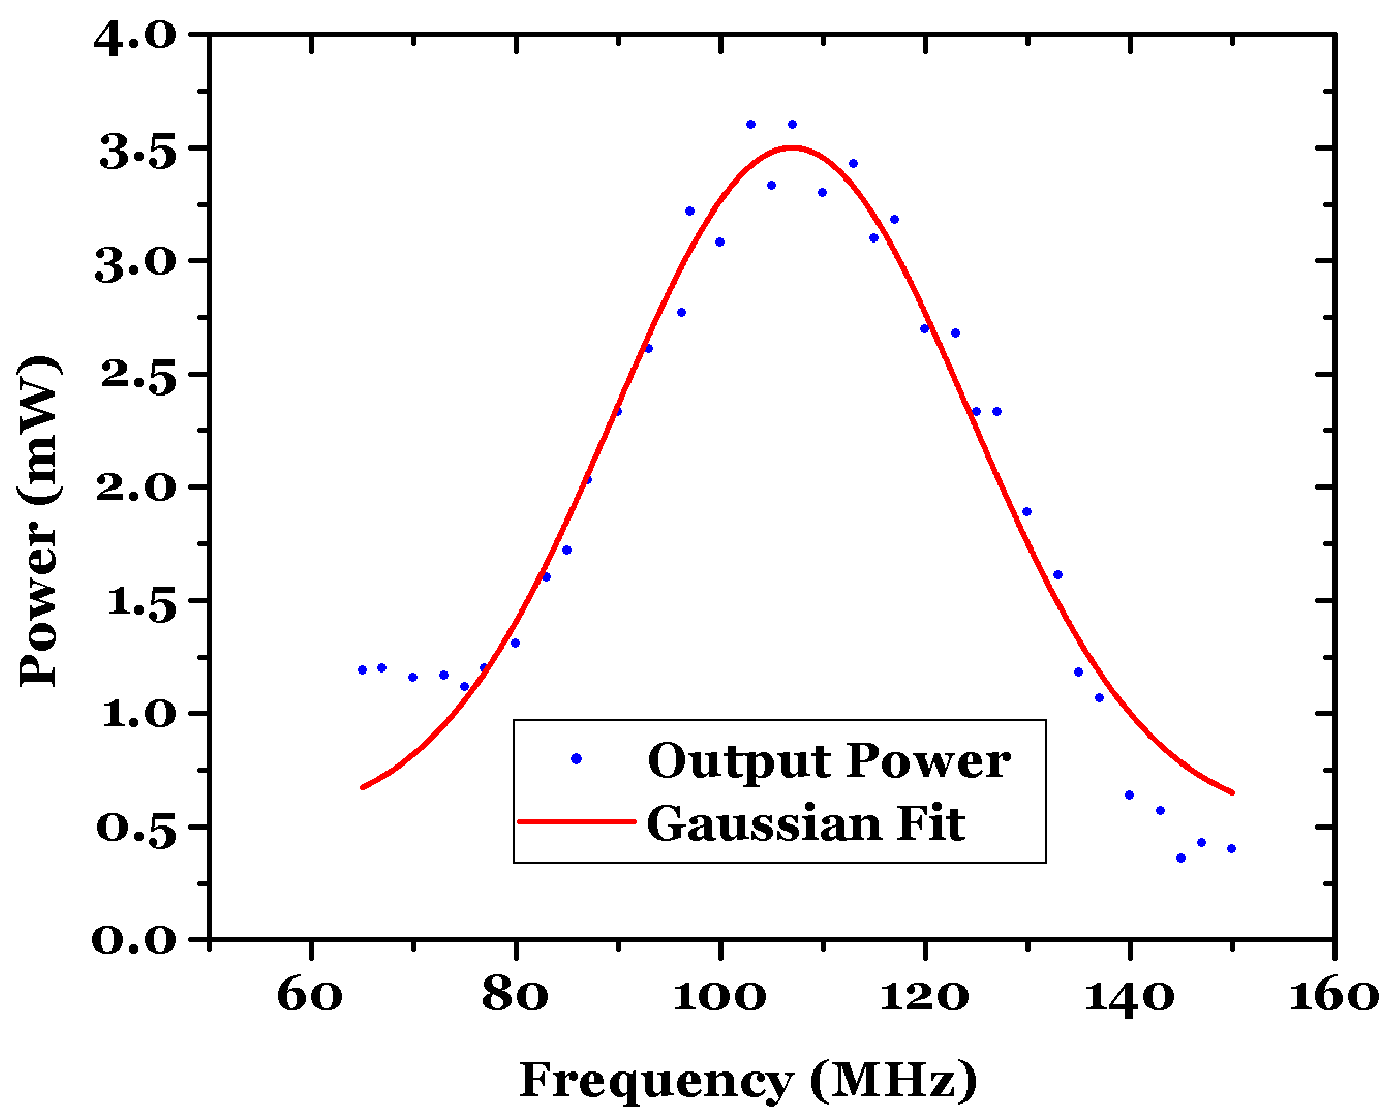
\includegraphics[height=2.5in]{figures/graph.png}
%
%    \caption[Optional: Short caption to appear in List of
%    Figures]{Full caption to appear below the Figure}
%
%    \label{figure1}
%\end{figure}

% +--------------------------------------------------------------------+
% |To create cross-references to figures, tables and segments
% |of text, LaTeX provides the following commands:
% |   \label{marker}
% |   \ref{marker}
% |   \pageref{marker}
% | where {marker} is a unique identifier.
% |
% | In the line above, we use \label{figure1} to mark a location
% | we wish to refer to later.  LATEX replaces \ref by the number of
% | the chapter, section, subsection, figure, or table after which the
% | corresponding \label command was issued. \pageref prints the page
% | number of the page where the \label command occurred.
% |
% +--------------------------------------------------------------------+

%\begin{table}
%
%% +--------------------------------------------------------------------+
%% | We include the command \begin{center} to center the table
%% | horizontally on the page.  Note use of the command \end{center}
%% | to turn off centering after the table is defined.
%% +--------------------------------------------------------------------+
%    \begin{center}
%
%% +--------------------------------------------------------------------+
%% | The table is created with this command
%% |
%% | \begin{tabular}[pos]{table spec}
%% |
%% | The "pos" argument specifies the vertical position of the table relative to
%% | the baseline of the surrounding text.  Use t, b, or c to specify alignment
%% | at the top, bottom, or center.
%% |
%% | The "table spec" command defines the format of the table
%% |   l for a column of left-aligned text
%% |   r for a column of right-aligned text
%% |   c for centered text
%% |   p{width} for a column containing justified text with line breaks
%% |   | for a vertical line
%% +--------------------------------------------------------------------+
%
%    \begin{tabular}[c]{|c|c|c|}
%        \hline
%        Column 1 Heading & Column 2 Heading & Column 3 Heading \\
%        \hline
%        Col 1 Row 1 & Col 2 Row 1 & Col 3 Row 1\\
%        Col 1 Row 2 & Col 2 Row 2 & Col 3 Row 2\\
%        Col 1 Row 3 & Col 2 Row 3 & Col 3 Row 3\\
%        \hline
%    \end{tabular}
%    \caption{Caption to appear below the table}
%    \label{table1}
%   \end{center}
%\end{table}

% +--------------------------------------------------------------------+
% | Replace \section headings below with the title of your
% | subsections.  LaTeX will automatically number the subsections 1.1,
% | 1.2, 1.3, etc.
% +--------------------------------------------------------------------+

\section{Los videojuego educativos y el E-Learning}
\label{seriousgames}

El e-Learning, también conocido en español con la terminología de Aprendizaje Electrónico, es aquello que, según Martín Hernández, engloba aquellas aplicaciones y servicios que, tomando como base las TIC, se orientan a facilitar el proceso de enseñanza-aprendizaje [1]. Este e-Learning surgió en un primer momento con la intención de facilitar el acceso a la información al mayor número de personas posibles, pero esto fue satisfecho rápidamente por sistemas muy simplificados de e-Learning que básicamente son grandes repositorios de información con unas pocas facilidades.

Este sector, sin embargo, está avanzando para que no haya tanta diferencia con los sistemas de educación tradicionales, intentando reducir la separación que se produce entre un profesor y un alumno cuando se realiza la educación mediante plataformas educativas en línea, añadiendo elementos de monitorización y seguimiento, elementos que fomentan la participación en comunidad como foros de trabajo, o añadiendo elementos de gamificación en los proyectos de aprendizaje que se desarrollan.

No obstante, estos sistemas de educación pese a ser mucho más dinámicos, permitiendo que los usuarios marquen su ritmo de aprendizaje, y presentarse con un enfoque diferente, que supone un grado de implicación personal en el que es el usuario el que decide realizar un aprendizaje, y no una imposición social, familiar o incluso personal; no dan la motivación suficiente a muchos estudiantes para continuar con la educación y no abandonarla. Es por ello que otro tipo de género de herramientas de e-Learning surgen, donde la motivación para aprender se adquiere a través del uso de la herramienta, y el aprendizaje suele ser una cualidad implícita que se adquiere por la utilización de la misma. Estos son los videojuegos educativos.

El abandono escolar es uno de los problemas más importantes actualmente. Según Prensky, los estudiantes son nativos digitales, personas capaces de interactuar con ricos dispositivos digitales como ordenadores, dispositivos móviles o videoconsolas. Esto difiere con las metodologías tradicionales de educación, en términos de interacción y contenido [2].

Por todo ello, los videojuegos educativos suponen un tema de estudio y desarrollo muy importante dentro de las diferentes tecnologías de e-Learning.

%In this paragraph, we want to refer to Fig.~\ref{figure1}
%mentioned at the beginning of this chapter.  We also refer to the
%Table~\ref{table1}.

\section{El Objeto de Trabajo}
\label{objetodetrabajo}

El objeto de trabajo de este proyecto se ha dividido en tres aspectos. En primer lugar la plataforma de desarrollo de videojuegos educativos eAdventure, la cual comienza a sufrir problemas de portabilidad debido a estar desarrollada en Java. En segundo lugar el videojuego Checklist, desarrollado en eAdventure y que se utiliza para formar a personal sanitario acerca de la utilización de la Lista de Verificación Quirúrgica. Y en tercer lugar, el motor de videojuegos Unity, que en contraposición a eAdventure, es ampliamente conocido por las facilidades que brinda a los desarrolladores para exportar sus proyectos en multitud de plataformas diferentes.

\subsection{eAdventure}
\label{eadventure}

Sobre eAdventure Los videojuegos educativos, a la hora de ser producidos, tienen tres grandes problemas a los que los productores del videojuego deben enfrentarse. Estos tres problemas son: 

En primer lugar, la dificultad de balancear la parte divertida y la parte educativa del videojuego. El correcto balance de ambos aspectos es necesario para el éxito del videojuego, pues, si los estudiantes no se divierten mientras juegan, lo mas probable es que terminen abandonando el juego, lo que echaría por tierra todo el esfuerzo de creación del videojuego; y por otra parte, si todos los esfuerzos son puestos en hacer la parte divertida del juego, es posible que el impacto educativo del mismo sea demasiado pequeño. Diversos autores como Dickey defienden que, los videojuegos enfocados en la historia, como cuentacuentos digitales, o aventuras gráficas point-and-click, son géneros que se adecuan mucho a las necesidades de los videojuegos educativos.

Las aventuras gráficas son un género conocido dentro del mundo de los videojuegos, con grandes títulos como Monkey Island, The Day of The Tentacle o, la franquicia española, Runaway. Tal es el grado de popularidad que tienen estos videojuegos que existen herramientas específicas para la creación de videojuegos de este género, como Adventure Game Studio, DAGE o Open SLUDGE. Sin embargo, todo este tipo de herramientas, pese a ayudar mucho a producir videojuegos de este género, pero no aportan funcionalidades específicas para los videojuegos educativos. De esta manera, eAdventure, aporta un enfoque específico orientado a los videojuegos educativos. 

En segundo lugar, el desarrollo de videojuegos es uno de los sectores dentro del desarrollo de software que supone un coste muy grande para su desarrollo, llegando a costar varios millones de dólares. En la última década, han surgido varios proyectos de videojuegos educativos cuyo presupuesto supera los cientos de miles de euros [2]. Sin embargo, con herramientas apropiadas que simplificasen el proceso de desarrollo del juego, y que además fuesen de bajo coste, se podría reducir el presupuesto necesario para desarrollar videojuegos educativos. Es por ello que eAdventure se presenta como una alternativa libre y gratuita para simplificar el desarrollo de videojuegos educativos. 

Y finalmente, en tercer lugar, el último problema que tienen los videojuegos, está relacionado con los problemas de distribución de un videojuego una vez que está desarrollado. Es frecuente encontrar que videojuegos están únicamente
disponibles en una plataforma o sistema operativo, por lo que gran cantidad de personas no pueden disfrutar de un videojuego, y por consiguiente, los desarrolladores no consiguen que sus videojuegos no tengan el efecto deseado.

Sin embargo, esta herramienta, como se mencionó en la introducción, está desarrollada en Java, y produce Applets standalone, que, pese a no necesitar ninguna instalación, necesitan de la maquina virtual Java para funcionar. La máquina virtual Java ha gozado de mucha popularidad a lo largo de los años, pero actualmente cada vez cuesta más encontrar dispositivos de uso cotidiano que dispongan de ella. Tanto es así que, sistemas operativos como Android, cuyo lenguaje de programación principal es Java, han construido su propia máquina virtual llamada Dalvik [3], la cual está siendo sustituida actualmente por ART [4], y que reemplaza completamente a la maquina virtual Java para la ejecución de programas desarrollados en dicho lenguaje.

Es por ello que el desarrollo analizado en este artículo se encarga de mejorar la capacidad de eAdventure para la distribución de juegos, desarrollando un intérprete capaz de visualizar un juego creado en eAdventure, en el motor de videojuegos Unity. 

%In this section, we refer back to text mentioned in
%Section~\ref{makereference1.1} on page~\pageref{makereference1.1}.

\subsection{Checklist}
\label{checklist}

Ante la pregunta ¿Que instrumento reduce el ratio de muertes y complicaciones en cirugía en más de un tercio? Pese a que pueda parecer que son los avances tecnológicos, la calidad de la medicina y de los utensilios, o la higiene en los hospitales, esta no es la respuesta. Estos factores han mejorado la medicina, y han logrado que avance hasta el punto de realizar operaciones que antes considerábamos impensables, ayudando a los médicos a detectar problemas mucho antes de que surjan y a monitorizar situaciones peligrosas. Pero es algo mucho mas sencillo lo que ayuda a evitar muertes y complicaciones, y esto es una simple lista que se realiza antes, durante y después de una operación. Esta lista tiene el nombre de Lista de Verificación Quirúrgica [5].

La Lista de Verificación Quirúrgica fue desarrollada por la Organización Mundial de la Salud en 2007 buscando identificar las normas mínimas de aplicación universal. Se construyó mediante el estudio de pacientes, cirujanos, anestesiólogos, enfermeras y expertos en seguridad de los pacientes a lo largo de dos años. En si, la lista está formada por simples comprobaciones que llevan muy poco tiempo de realizar, y no debe ser una carga para el equipo quirúrgico, pues ellos ya tienen una labor muy importante que llevar a cabo.

El videojuego Checklist surge para concienciar y educar acerca de la correcta aplicación de la Lista de Verificación Quirúrgica, mostrando, tanto los beneficios de aplicarla correctamente, como las consecuencias de una mala aplicación. Se desarrolló en la UCM, por el grupo de investigación eUCM junto con la Facultad de Medicina de la UCM, el Hospital Doce de Octubre y el Massachusetts General Hospital [6].

Este juego está desarrollado utilizando eAdventure, y por consiguiente es del género Aventura Gráfica, más concretamente, una en Primera Persona, en la que el jugador no maneja a un personaje dentro de un juego, sino que ocupa el lugar del protagonista, quien toma uno de los diferentes roles que se ofrecen y que participan dentro de un quirófano, y realiza participación en una operación en tres situaciones diferentes: Antes de inducir la anestesia al paciente, antes de la primera incisión en la piel, y antes de que el paciente se marche de la sala de operación. Asimismo, dentro del videojuego suceden diferentes eventos que se dan de forma aleatoria, como una incisión mal marcada, o un compañero que no coopera.

El paquete ejecutable está disponible en Windows, Mac OS X y Linux, en versiones de 32 y 64 bits. Adicionalmente, el Applet Standalone se puede encontrar en el repositorio en Sourceforge de eAdventure, y permite la ejecución mediante el uso de la máquina virtual Java. Sin embargo, la ejecución de dicho juego en Tablets Android e iPad no está disponible, por ello se realiza la adaptación de dicho juego a Unity 

\subsection{El motor de videojuegos Unity}

Los motores de videojuegos son herramientas que permiten y facilitan la creación y desarrollo de un videojuego. Estos, dan la funcionalidad básica de proveer de un entorno gráfico para la representación del videojuego, así como un motor físico con detección de colisiones, junto con un bucle principal que se encarga de procesar y ceder tiempo de procesamiento para cada uno de los elementos del videojuego.

Unity es un motor de videojuegos caracterizado por ser capaz de producir videojuegos para multitud de plataformas, entre las cuales encontramos Windows, OS X y Linux, junto con los mas frecuentes sistemas operativos móviles y de tabletas, como Android e  iOS, tanto iPad como iPhone, además de videoconsolas como PlayStation 3, PlayStation Vita, Wii, Wii U, etc. Esta facilidad para producir videojuegos en múltiples plataformas, así como su licencia gratuita para los desarrolladores independientes, y pequeñas startups que no tienen presupuesto para pagar las costosas licencias de los motores de videojuegos, hacen de este motor una opción muy elegida por gran número de desarrolladores que quieren llegar al mayor número de personas con el menor esfuerzo posible.

Asimismo, otras de las características de este motor incluyen la, ampliamente utilizada en videojuegos, arquitectura basada en componentes, en la que los objetos se componen de distinta manera dependiendo de sus necesidades en cada momento, permitiéndoles mutar o adquirir un comportamiento adicional si se requiere; en contraposición a la arquitectura orientada a objetos, en la que los objetos adquieren una funcionalidad al implementar una interfaz o heredar de una clase de una jerarquía superior, así como adquirir funcionalidad mediante la implementación de si misma. Esta arquitectura permite tener objetos más dinámicos, así como facilitar la reutilización de código gracias a la incorporación del mismo componente en varios objetos, sin embargo supone un cambio de paradigma en la programación, y requiere conocer tanto el funcionamiento de Unity, la comunicación entre sus componentes, así como el complejo ciclo de vida que compone cada Tick de juego [7].

En Unity, cada objeto que toma partido dentro de la escena, está constituido por un GameObject y todas aquellas componentes asociadas, extendiendo a la clase MonoBehabiour, así como una componente Transform que le permite orientarse y deformarse en la escena, y una


\section{Estado del Arte}
\label{estadodelarte}

\section{Metodología de desarrollo}
\label{metodologiadedesarrollo}

Una parte crucial de todo proyecto de ingeniería del software es la metodología de desarrollo que se ha utilizado para su construcción. La metodología determina el proceso de generación del software, pudiendo ser una metodología más lineal como el Proceso Unificado de Desarrollo de Software, o un desarrollo en Cascada, o metodologías basadas en la iteración, como el modelo en espiral de Boehm, o un desarrollo incremetal. Sin embargo, la mayor parte de estas metodologías están pensadas para coordinar a grandes equipos en procesos de desarrollo de larga duración. Por consiguiente, existen metodologías de desarrollo más apropiadas para pequeños equipos que, debido a su configuración de personal y a la rápida comunicación entre miembros, entre otros factores, consiguen que el desarrollo de dicho software sea mucho más ágil.

Asimismo, este proyecto, como muchos de los Trabajos de Fin de Máster, consta de una amplia parte dedicada a la investigación, aprendizaje de nuevas tecnologías, o del desarrollo de prototipos para verificar si esa es la manera más apropiada de hacerlo.

Es por ello que, para desarrollar este proyecto se ha utilizado una metodología de desarrollo ágil, basada en prototipos, en la que se realizan múltiples iteraciones, tanto sobre cada uno de los componentes que conforman el sistema, como sobre el sistema en sí mismo, realizando tres grandes iteraciones sobre el mismo: 

\begin{itemize}
	\item 
	Una primera iteración para estudiar y analizar los videojuegos de eAdventure, así como para interpretar dichos paquetes e intentar representarlos, aprendiendo de los resultados obtenidos mediante el primer prototipo.
	\item
	Una segunda iteración generando un mejor diseño de la aplicación, nuevas interfaces, refactorización de clases y código replicado,  
\end{itemize}

Como 



Esta metodología ha influido muy fuertemente en el desarrollo de este proyecto, 



% +--------------------------------------------------------------------+
% | Uncomment the lines below to add additional chapters.  Name the
% | files chapter2.tex for Chapter 2, chapter3.tex for Chapter 3, etc.
% +--------------------------------------------------------------------+

% +--------------------------------------------------------------------+
% | Sample Chapter 2
% +--------------------------------------------------------------------+

\cleardoublepage

% +--------------------------------------------------------------------+
% | Replace "This is Chapter 2" below with the title of your chapter.
% | LaTeX will automatically number the chapters.
% +--------------------------------------------------------------------+

\chapter{Comenzando con el Proyecto}
\label{makereference2}

Tras obtener el videojuego Checklist en su versión ejecutable, el cual se puede descargar a través del repositorio de eAdventure en Sourceforge, se realizó un estudio. Se completó el videojuego en repetidas ocasiones intentando buscar la aleatoriedad que aparecía descrita en los documentos del proyecto, y analizar a fondo el funcionamiento del mismo. 

En una primera instancia parece un videojuego sencillo, con mecánicas muy simples, apenas reglas para el desarrollo, más allá de las que se nos imponen circunstancialmente en alguna de las escenas en las que no podremos avanzar sin tener la atención del equipo. Sin embargo, el juego esconde una mayor complejidad, pues tus decisiones dentro del juego te llevarán a alcanzar un final diferente cada vez que el juego es completado. El análisis de la no linealidad del juego, así como la aleatoriedad de algunos de sus elementos, como la no colaboración de miembros del equipo, o la posibilidad de que algunas de las labores que se comprueban en la Lista de Verificación Quirúrgica estén mal realizadas, hacen que implementación del videojuego no sea tan sencilla al perder la linealidad. Asimismo, el videojuego está compuesto por multitud de recursos de gran variedad de tipos, entre los que encontramos imágenes, animaciones, y textos. 

La obtención de los recursos del videojuego se realiza mediante la extracción del paquete ejecutable standalone producido por eAdventure. Dicho paquete es un archivo “.jar”, disponible en el repositorio de SourdeForge de eAdventure, más concretamente en su carpeta Games1. Mediante la extracción de dicho paquete, no sólo se obtienen los recursos del juego. El paquete “.jar” está compuesto por: Una carpeta “Assets” donde se encuentran los recursos pertenecientes al juego en concreto, una carpeta “gui” que contiene recursos que utilizan los juegos de eAdventure y que son genéricos para todos ellos, como botones, cursores para el ratón, e iconos; además, dentro del paquete se incluye el núcleo de eAdventure, intérprete capaz de ejecutar el juego, junto a multitud de librerías y codecs para la decodificación de vídeo. Finalmente, en la raíz de este fichero se encuentran los archivos de definición del juego, en formato XML junto a las DTD que permiten la interpretación correcta de dichos ficheros. Adicionalmente, este paquete es interpretable por eAdventure, por lo que permite el estudio del videojuego de una forma más visual y aclaratoria. Abrir el paquete con esta plataforma y dedicar un tiempo a analizar cómo se han construido algunos de los elementos que lo forman permite una mejor elección de la estrategia que se llevará a cabo para la implementación de dicho juego en Unity.

Cabe destacar la existencia de ficheros de Animación dentro de la carpeta “/assets/animation/”. Estos ficheros son el formato “.eaa”, y son generados por eAdventure. Aunque en primera instancia parezcan un formato propio de dicha plataforma, estos ficheros son interpretables por un editor de texto, y son descripciones en XML de cómo se debe realizar la animación. Asimismo, la DTD de dicho fichero XML se puede encontrar en la raíz de archivos del videojuego. 

Un análisis en profundidad de los ficheros de definición del videojuego, es decir, de los ficheros XML, explica que, dentro de dicho fichero XML podemos encontrar las definiciones de los siguientes elementos: Escenas, Personajes, Objetos, Objetos de Atrezo, estados de la máquina de estado, Macros, Efectos, Acciones… Además, dentro de dicho archivo se especifican todas aquellas condiciones que, dependiendo del estado del juego, causan la representación de escenas de una forma diferente, así como las diferentes respuestas contextuales que podemos obtener al interactuar con algún personaje en un momento concreto, junto a los Grafos de diálogo. Cabe destacar que dichos archivos de definición alcanzan un gran tamaño, siendo, en el caso de Checklist, de una longitud aproximada de 10.000 lineas de código, sin contar los archivos de animaciones que también definen más elementos del juego. 

Encontrar dichos grafos separados del código plantea un dilema a la hora de la implementación. Se nos presentan dos opciones. La primera opción consiste en transcribir los diálogos a mano e incluirlos dentro del código del programa, y la segunda opción consiste en mantener diálogos y textos en general, separados del código del programa. Ambas opciones son válidas y ambas se realizan en la implementación de cualquier tipo de software. Un análisis breve nos lleva a las siguientes conclusiones: 

\begin{itemize}
	\item 
	Transcribir el texto a mano e incluirlo dentro del código del programa es laborioso, y ese tiempo es mucho más valioso invertirlo en realizar un buen diseño de la arquitectura del videojuego. En general, el coste del salario de cada trabajador es más alto cuanto más compleja sea la labor que desempeña, y mayor sea su cualificación, es por ello que el precio de un arquitecto de software y el de un programador no es el mismo. Por ello invertir el tiempo en realizar una labor de más alto nivel, reducirá costes
	\item 
	Pese a que existen herramientas para la localización de programas mediante el análisis del código en busca de fragmentos de texto para traducir [8], Incluirlo dentro del código del programa, más concretamente dentro del código de cada uno de los personajes, dificulta esta tarea de localización, teniendo que volver a producir el juego una vez se haya traducido y sus elementos se hayan adaptado a la cultura en la cual se va a desplegar dicho programa. 
	\item
	Finalmente, la obtención de los textos de un archivo externo permite la reutilización del software que desempeñe esa función, para otros proyectos similares, pudiendo realizar la interpretación de textos para otros videojuegos de eAdventure. 
\end{itemize}

Es habitual encontrar los textos de un programa separados del código. Uno de los fundamentos de la construcción de Web consiste en mantener el HTML con únicamente datos de contenido, y CSS con la definición acerca de la representación de dichos datos [10]. Otro ejemplo es el de los programas desarrollados para Android, los cuales disponen de un archivo llamado “strings.xml”, junto a muchos otros archivos similares, en donde se incita a los desarrolladores a incluir todos los textos del programa, como los títulos de los menús, los nombres de los campos de los formularios, o las descripciones de algunos elementos[9]; y que facilita la traducción del programa cuando un usuario de la Google Play Store de otro país instala dicha aplicación. En la reconstrucción de Checklist sobre Unity se opta por mantener separados el código y los textos, y realizar un análisis con la librería System.Xml de C\#, extrayendo el contenido de los diálogos de los ficheros de definición del juego. 

Analizando en profundidad el último punto de la anterior lista de conclusiones acerca de mantener el código separado del texto, remarcando la posibilidad de reutilizar dicho software, y pudiendo obtener de los archivos de definición del juego, todas las descripciones de los elementos, junto a los diálogos, efectos, condiciones, macros, personajes, etc. Se plantea la opción de poder generar una herramienta capaz de interpretar cualquier juego de eAdventure, sin ninguna implementación específica, y “reproducir” dicho juego en Unity. 

La implementación de dicha herramienta capaz de interpretar cualquier juego es más costosa frente a una implementación centrada y enfocada en Checklist, pero, la realización de dicho esfuerzo ahorrará mucho más esfuerzo en el futuro cuando se desee aprovechar muchos de los otros juegos generados con eAdventure. 

Por todo ello, se tomó la decisión de realizar un intérprete de juegos de eAdventure, y,habiendo alcanzado dicho punto, no mucha más información es necesaria para comenzar con el diseño e implementación del videojuego. 

%\section{Page Number References}
%\label{makereference2.1} I should also be able to refer to a
%specific page number, such as page~\pageref{makereference}.  Of
%course, I'll need to have a slash label command and a unique name
%in each section that I want to be able to refer to later in the
%text.
%
%\section{Referring to Sections Within Chapter 1}
%\label{makereference2.2} Now, I'm going to refer to different
%sections within Chapter 1. I gave an example of a figure in
%section~\ref{makereference1.1} and an example of a table in
%section~\ref{makereference1.2}.  In
%section~\ref{makereference1.3}, we looked at examples of
%bibliographic citations.

\chapter{Primera Iteración: Prototipo inicial}
\label{primeraiteracion}

\section{Arquitectura del Proyecto}
\label{it1arquitectura}
La arquitectura del proyecto está caracterizada por la dinamicidad y capacidad para adaptarse de sus clases. Permitiendo que tomen un rol u otro dependiendo de las clases que las definan. Es decir, una clase personaje debe adaptarse al rol de personaje que le toque interpretar, y al contexto que le pone dentro de la escena. Además, debe seleccionar el recurso que lo represente que cumpla con las condiciones que se den en ese momento dentro de la escena. Finalmente debe permitir la interactuación y ejecución de efectos que están asignados a si mismo.

En esencial, esto se puede explicar con el diagrama de clases muy simplificado de la figura 3. Este diagrama fue generado en esta iteración del proyecto, por lo que su formato es muy diferente al resto de diagramas que se muestran en posteriores iteraciones.

\begin{figure}[htb]
	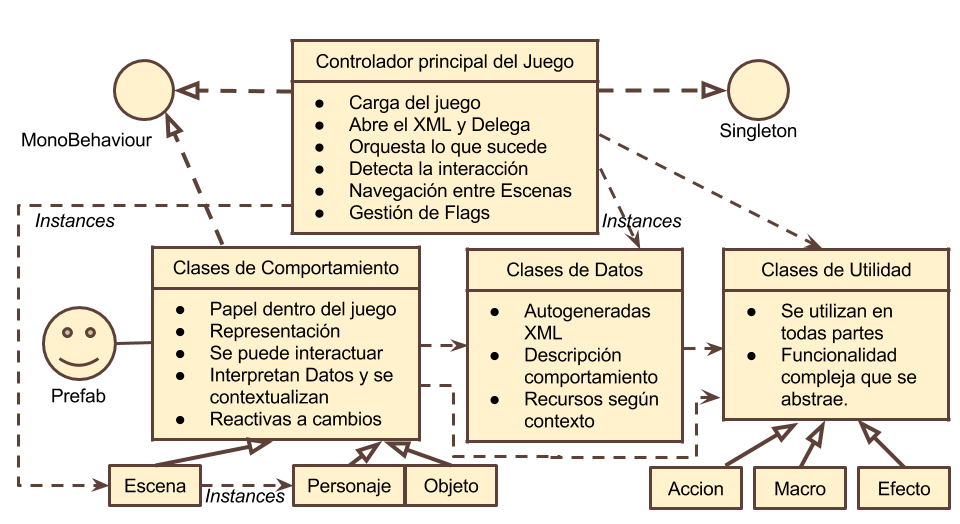
\includegraphics[height=3.5in]{figures/arquitecturait1.png}
	\caption[Arquitectura simplificada - Prototipo 1]{Diagrama de clases simplificado de la arquitectura de clases de la primera iteración del proyecto.}
	\label{arquitecturait1}
\end{figure}

En la figura \ref{arquitecturait1} hay varios elementos que no son comunes en un diagrama de clases. El primero de ellos es la "Cara sonriente" que aparece a la izquierda con el texto \textit{Prefab} debajo de el. Este \textit{Prefab} es un elemento en Unity3D que resume el concepto de Objeto Prefabricado, y que, contiene, una representación tridimensional, junto a todas las componentes y comportamientos que definen dicho objeto. Por otra parte la interfaz \textit{MonoBehabiour} no es una interfaz, sino una clase abstracta, y esta, provee a los elementos que la extienden de la habilidad de ser componentes para los objetos de la escena. Dicha clase contiene varios métodos como Start(), Awake() o Update() que permiten a estos comportamientos inicializarse, actuar, y en esencia, tener una fracción de tiempo para realizar acciones dentro de la escena de Unity3D.

En la figura \ref{arquitecturait1} encontramos cuatro tipos de clases:

\begin{itemize}
	\item El controlador principal del juego.
	\item Las Clases de Datos
	\item Las Clases de Comportamiento: Escenas, Personajes, Objetos, Salidas, etc...
	\item Las Clases de Utilidad: Acciones, Efectos, Macros, Secuencias, Diálogos, etc...
\end{itemize}

Todas las clases que se presentan en este primer prototipo han sufrido cambios muy grandes o totales tanto en su código, como en su funcionalidad. Algunas de ellas han desaparecido, surgiendo clases nuevas que realizan su funcionalidad, otras se han transformado completamente o han sido asumidas por otras, y finalmente, otras han surgido de la generalización y refactorización de código.

\subsection{Controlador Principal de Juego}

El controlador principal de juego, implementado con una clase de nombre Game, se encarga de, en primer lugar, comenzar la carga del juego, comenzando a explorar el XML y delegando en las Clases de Datos su propia interpretación, así como orquestar lo que sucede dentro del juego, detecta la interacción por parte del jugador y notifica a aquellos elementos cuando se interactúa con ellos, realiza la navegación entre escenas cuando es necesario, y controla el estado de los interruptores que controlan las condiciones para la contextualización de cada escena en su momento apropiado.


Implementa el patrón Singleton, pues sólo una instancia es necesaria para el control.

\subsection{Clases de Datos}

Las clases de datos se encargan de generarse a partir de un elemento del fichero XML y sirven de descripción para una Clase de Comportamiento para representarse y interactuar de la forma correcta en cada momento. A través del documento XML realizan una lectura del mismo mediante la librería de c\# System.Xml, y rellenan sus atributos a partir de la especificación en dicho XML. Asimismo implementan funciones útiles como la obtención de un paquete de recursos apropiado según el contexto.

Existe una clase de datos por cada Clase de Comportamiento, aunque también existen clases de datos auxiliares mucho más pequeñas y que apenas aportan funcionalidad, siento meros contenedores de datos.

\subsection{Clases de Comportamiento}

Las clases de comportamiento son aquellas clases que juegan un papel dentro del videojuego y participan de forma activa en la representación del mismo. Dentro de esta categoría encontramos a las Escenas, los Personajes, los Objetos, las Salidas de las escenas, así como los objetos de atrezo y todos aquellos elementos que tienen una representación virtual en el videojuego. 

Cada una de estas clases heredará de la clase de Unity \textit{MonoBehabiour}, que indica, como se explica en la sección \ref{it1arquitectura}, que dicha clase es un comportamiento y se puede asignar como componente a un elemento de la escena. Cada una de ellas tiene un objeto de datos que debe interpretar. Esta clase de comportamiento recibirá estímulos por parte del controlador principal del juego cuando el jugador interactue con ellas. Este paso intermedio es necesario ya que hay momentos en los que el controlado principal debe evitar la interacción del jugador con dichos elementos por encontrarse en mitad de un diálogo. Con este estímulo, la clase de comportamiento gestiona las diferentes interacciones que tenga el usuario con si mismo.

Finalmente, estas clases se encapsulan dentro de un \textit{Prefab}, formando parte como componente de un objeto tridimensional, junto a otras componentes.

\section{Detalles de la implementación}

Existen algunas cuestiones cruciales y generales acerca de cómo se realizó la implementación de diversas mecánicas que eran necesarias para que el juego funcionase.

Algunas de estas decisiones cruciales son, por ejemplo, la decisión de \textit{reRenderizar}\footnote{Renderizar es el proceso de generar una imagen, mediante el cálculo de la iluminación, a partir de un modelo 3D. En este caso se refiere a regenerar la representación de la escena.} la escena junto con todos sus elementos cada vez que un \textit{Flag}\footnote{Una Flag, bandera en Inglés, es un elemento que se utiliza para establecer hitos dentro del juego, como haber hablado con un personaje, o haber fallado una respuesta.} o una Variable de entorno cambia. Esto puede tener efectos devastadores si nuestra escena tiene elementos que han sido modificados por el jugador en un momento determinado, pero en el caso del videojuego Checklist, no existen dichos elementos, por lo que, cada vez que se activa un flag, en lugar de notificar a cada uno de los elementos, se \textit{renderiza} de nuevo la escena entera.

Esta decisión se tomó debido a que, pese a que existía la opción de implementar el patrón Observador-Observable, y hacer que todos los elementos de la escena fueran observadores y fuesen notificados cuando el estado del juego cambie, es frecuente que ocurra que, un elemento de la escena que en ese momento no tiene representación física, deba de reaccionar a este cambio en el estado del juego, y debido a que nunca recibirá la notificación, porque no existe, nunca aparecería.

No obstante esta decisión de volver a generar la escena, pese a que se mantiene, evolucionará en la siguiente iteración del proyecto, permitiendo al usuario modificar los elementos que se hallen dentro de la escena, guardando en un diccionario, referencias a los contextos dentro de las mismas. Por el momento no se han encontrado problemas de rendimiento con esta decisión, ya que las escenas, en general, suelen estar formadas por pocos elementos. Si se encontrasen dichos problemas, se desarrollaría un método más eficiente.

Otra de las decisiones cruciales de la implementación consistió en decidir si generar un \textit{SecuenceManager} que gestiona por completo las secuencias que se dan, como efectos, o diálogos; o por otra parte, hacer que las propias clases de \textit{GraphConversation} y \textit{Effect} fuesen capaces de ejecutarse por sí solas.

Después de comenzar con la implementación del \textit{SecuenceManager}, y construir una pila de secuencias, se vió que sería considerablemente complejo recordar datos contextuales acerca del estado de cada secuencia en caso de que fuese necesario parar la ejecución, y se decidió que era más sencillo que cada secuencia recordase por sí misma su posición.

En una sección posterior se detallan en profundidad los detalles de la implementación de las clases Conversation y Effect, dos clases que implementan la interfaz Secuence, y que permiten ser ejecutadas por si mismas.

\subsection{Sobre la clase Game}

La clase Game es el Controlador principal del juego, y por ello realiza todas las funciones anteriormente descritas.

Sus funcionalidades se podrían categorizar en 4 apartados:

\begin{itemize}
	
	\item En primer lugar, y en la parte de más arriba del código se encuentra la gestión del \textit{singleton} y del acceso a las variables de entorno. Es decir, se facilita el acceso a las \textit{Flags} del juego, a las Variables, a la obtención de \textit{Macros}, Las especificaciones de los diálogos, etc. Esta parte es vital para el control del juego, y su estado.
	
	\item En segundo lugar, tras todas estas funciones, se encuentra el cargador de juego. Se ha implementado mediante el uso de un \textit{Thread}\footnote{Un Thread, en programación, es un proceso que se ejecuta de forma paralela a la ejecución del programa, por lo que permite la realización de múltiples tareas simultáneamente} que permite visualizar el estado de la carga del juego mientras esta se realiza, y, como Unity no permite cargar recursos con \textit{Resources.Load()} fuera del bucle principal del juego, se utiliza la librería del sistema \textit{System.IO.File} para leer directamente los ficheros y generar texturas con ellos. Aquí entra en juego la clase \textit{Texture2DHolder} de la que se realiza una explicación posteriormente.
	
	Este cargador prepara el fichero XML utilizando la librería del sistema System.Xml, y lo secciona en pequeños bucles, uno por cada elemento del juego, es decir, uno por personajes, otro por objetos, otro por escenas, etc. Cuando termina la carga, se cambia el estado de la clase \textit{Game} para comenzar con la visualización del juego.
	
	\item En tercer lugar, se encuentran determinadas funciones útiles que realizan tareas variadas como \textit{RenderScene}, para pintar una escena o \textit{Execute} para comenzar la ejecución de una secuencia, junto con la función \textit{Update()} donde se realiza parte del control del juego, junto con la gestión del click del usuario, donde bloquearemos dicho click, notificaremos al elemento clicado o simplemente extraemos las acciones disponibles de dicho elemento, dependiendo del estado del juego.
	
	\item Por último, y al final del código, se encuentra otra parte de interacción, junto con el pintado de la interfaz. Para la interfaz se ha generado una \textit{GUISkin}\footnote{Una GUISkin es un fichero de especificación de datos de Unity que contiene datos acerca de los elementos de la interfaz, como el tamaño de la fuente, colores de los fondos, o imágenes de los botones.} propia que se modifica en función del tamaño de la pantalla para hacerse más grande o pequeña dependiendo de su proporción. Para el pintado de la interfaz se ha utilizado \textit{GUILayout}, clase que facilita métodos para representar una interfaz, ya que se conocía su funcionamiento de haberla utilizado en proyectos anteriores, y era sencillo de implementar.
	
	Esta GUI, además de adaptarse, se ha preparado para que se posicione correctamente utilizando \textit{Camera.current.WorldToScreenPoint()}, es decir, que transforma los puntos del mundo tridimensional, a unas coordenadas de cámara, y mediante una serie de transformaciones, se colocan los cuadros en su lugar, evitando que estos cuadros de diálogo se salgan de la pantalla cuando un personaje habla desde uno de los extremos.
\end{itemize}

Esta explicación cierra, por encima, todos los elementos importantes de la implementación de la clase Game. Debido a que esta implementación no es la final, no se incluyen explicaciones más detalladas ni diagramas.

Esta clase es una de las clases que ha sufrido una mayor evolución en la segunda iteración, ya que, pese a que sigue controlando la interacción por parte del usuario, ya no realiza la lógica de dicha interacción en el bucle \textit{Update()}, sino que, simplemente delega en los diferentes elementos interactuados para que sean ellos los que realicen la lógica de su interacción. Asimismo, la gestión de la interfaz ha sido delegada en la clase \textit{GUIManager}, con un nuevo y rediseñado sistema de burbujas.

\section{Sobre las Clases de Datos}

Existen multitud de clases de datos dentro del código del programa, aunque todas se parecen bastante entre sí, por lo que se explicarán la mayoría de ellas en conjunto.

\begin{figure}[htb]
	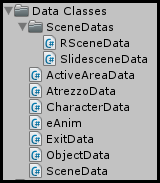
\includegraphics[height=2.5in]{figures/it1/dataclasses.png}
	\caption[Clases de Datos - Prototipo 1]{Vista de carpeta de las clases de datos implementadas en la primera iteración.}
	\label{dataclassesit1}
\end{figure}

Estas clases se auto-generan analizando un \textit{XmlElement} que reciben en su constructor, y por lo general no aportan funcionalidad, salvo excepciones como la función \textit{Check()} que implementan la mayor parte de recursos para verificar si se cumplen todas las condiciones para que dicho recurso pueda ser utilizado.

La mayor parte de clases de datos contienen:
\begin{itemize}
	\item Una serie de Recursos: con soporte de videos y animaciones (implementadas con la clase eAnim y eFrame). Algunas clases implementan su propia clase para manejar sus recursos con Condiciones, como CharacterData con su CharacterResource, o SceneData con su SceneResource, aunque muchas otras simplemente utilizan diccionarios de tipo Dictionary<string,Texture2DHolder> Resources.
	
	\item También tienen una serie de condiciones ante las que decidiran representarese o no, estas condiciones son gestionadas mediante la clase Condition.
	
	\item Algunas clases de datos, además de Recursos y Condiciones, también tienen Efectos que se realizan al interactuar con ellas, o un listado de Acciones que se muestra como un menú contextual al interactuar con ellas.
\end{itemize}

Particularmente, existen algunas anomalías en las clases de datos, como son las clases que implementan la interfaz \textit{SceneData} la cual contiene, además de Recursos como todas las demás, gran variedad de objetos \textit{ItemReference}, los cuales contienen una referencia a un elemento de la escena (ya sea un personaje, objeto o una salida) y la contextualización del mismo, es decir, su posición en ese momento, las condiciones que tienen que darse para que ese elemento aparezca o no, etc.

La creación de dicha interfaz fué necesaria debido a que existen multitud de tipos de escenas. En este caso se han implementado 2 tipos de escenas que eran necesarias para el videojuego \textit{Checklist}, las \textit{RScene}, abreviando \textit{Regular Scene}, que son escenas normales sobre las que jugar, donde se representan personajes, objetos, salidas, áreas activas; y las \textit{Slidescene}, que son escenas con una sucesión de imágenes en su interior a modo de \textit{Slides} como si de una presentación se tratase.

Finalmente comentar que, algunas clases de datos como los \textit{ObjectData} o los \textit{ActiveAreaData} tienen un elemento llamado \textit{InfluenceArea} el cual no se ha implementado, y que permite que un objeto o un active área sea mucho más grande que su area de interacción, la cual está formada por una sucesión de puntos que generan al final un polígono. Esto permite que pueda haber un objeto con formas irregulares e interactuar con él sólo en las zonas de real contacto con la imagen. Por lo que todas nuestras áreas de influencia serán rectangulares.

Esta Área de Influencia, sin embargo, en la siguiente iteración del proyecto sí que ha sido implementada, mediante la utilización de librerías de triangulación de polígonos irregulares de cualquier tipo, y la transformación de dichos polígonos en Mallas tridimensionales. La explicación de dicha transformación será realizada en la siguiente iteración.

Finalmente, la clase eAnim tiene una peculiaridad, y es que en versiones antiguas de eAdventure, las animaciones se generaban a partir de secuencias de imágenes en la carpeta animations, carpeta utilizada para el almacenamiento de las imágenes que forman las animaciones.

Es decir, existen animaciones formadas de la siguiente manera: “anim\_01.png”, “anim\_02.png” y estas están especificadas en el fichero de especificación del juego de eAdventure como “/animaciones/anim”. Esto supone dos problemas. El primero consiste en identificar cuál es el formato del fichero de imagen, por lo que existe una lista de tipos disponibles y se intenta encontrar un archivo que satisfaga tanto el nombre de la animación, como el formato correspondiente. Y en segundo lugar, no se sabe cuántos archivos hay, lo que hace que debas iterar hasta que no encuentres fichero.

Por otra parte, el nuevo formato de animaciones está definido en ficheros XML llamados “.eaa” que son mucho más sencillos de recorrer y contienen más información acerca de cada fotograma de la animación.

\section{Sobre las Clases de Comportamiento}

De manera similar al apartado anterior, se explicará el funcionamiento de la mayor parte de clases de comportamiento, puntualizando detalles acerca de algunas de dichas clases en concreto, como \textit{Character} o \textit{eObject}, que tienen comportamientos aislados como la gestión de fotogramas o la necesidad de cambiar cuando el usuario va a interactuar con ellos.

\begin{figure}[htb]
	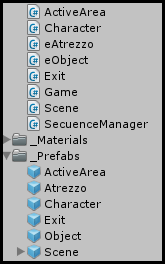
\includegraphics[height=3in]{figures/it1/behaviourclasses.png}
	\caption[Clases de Comportamiento - Prototipo 1]{Vista de carpeta de las clases de comportamiento implementadas en la primera iteración, junto a sus Prefabs.}
	\label{dataclassesit1}
\end{figure}

Las clases de comportamiento son todas herederas de \textit{MonoBehabiour} por lo que se asignan a objetos dentro de la escena, y luego estos objetos se guardan en forma de \textit{Prefabs}, cada una a uno individualmente. Estos \textit{Prefabs} suelen ser muy sencillos, en su mayoría constituidos únicamente por un \textit{Quad}\footnote{Un Quad es una malla tridimensional compuesta por un plano, una de las mallas más simples.}, al cual se le cambia la textura con \textit{this.GetComponent<Renderer>().material.mainTexture}, y posteriormente, mediante la información de dicha textura, se aplican modificaciones escalando el Quad. 

Todas estas clases de comportamiento son la representación de algún elemento de la escena, y por ello tienen en su interior los siguientes elementos:

\begin{itemize}
	\item En primer lugar una clase de datos asignada que será el “Guión” de nuestra clase para enrolarse. Es decir: una clase \textit{Character} contendrá dentro una clase \textit{CharacterData}, o una clase \textit{eObject} (la letra e era necesaria porque la clase \textit{Object} ya existe en el espacio de nombres, y proviene de juntar eAdventure con \textit{Object}), contiene una clase \textit{ObjectData}.
	
	\item En segundo lugar, aunque no todas la tienen, una \textit{ItemReference}, que utilizan para contextualizarse. Un \textit{character} no sería capaz de conocer su posición dentro de la escena si no tuviera un \textit{ItemReference} para poder contextualizar, y tampoco sabría si ese es su momento de aparecer en la escena, o si no debe aparecer más.
	
	\item Por último contienen aquellas funciones que son necesarias para su correcto funcionamiento.
\end{itemize}

\subsection{Detalles de la clase Character}

La clase \textit{Character} contiene una serie de comportamientos necesarios y características específicas que hacen que sea diferente a las demás, pues tiene animación y ha de ir cambiando el fotograma que la representa con el paso del tiempo, por lo que en su función de comienzo de la ejecución, \textit{Start()}, selecciona la animación que cumple todas las condiciones, y establece el primer fotograma, y en su función de actualización del estado, \textit{Update()}, va cambiando su fotograma con la funcion \textit{ChangeFrame()}.

Esta función \textit{ChangeFrame()} accede al \textit{renderer}\footnote{El renderer, en Unity3D, es la componente de los objetos que tienen representación en la escena, que define cómo se representan en la misma, con características como los materiales que las conforman, las texturas, las mallas tridimensionales, y otros elementos.} y cambia su textura además de actualizar determinadas variables de control, que establecen cuando deberá realizarse el próximo cambio de fotograma, o el fotograma que se está representando actualmente.

\subsection{Detalles de la clase eObject, Exit y ActiveArea}

Estas tres clases tienen la peculiaridad de que deben ser reactivas a interacción por parte del jugador, y mostrar algún cambio en su representación cada vez que el jugador pase el puntero del ratón por encima de ellas. Esto se implementó utilizando las funciones que facilita la clase \textit{MonoBehaviour}, I y \textit{OnMouseExit()} y que reciben el evento del puntero cuando este entra en su área de reacción y cuando sale de la misma.

Cada una de las tres clases que son reactivas a este evento realiza una acción diferente, donde, el \textit{eObject} cambia su imagen y, por otra parte, \textit{Exit} y \textit{ActiveArea}, acceden a su material para cambiar su color, volviéndose de color rojo la representación de \textit{Exit}, y de color verde la representación de una \textit{ActiveArea}.

Adicionalmente, la clase \textit{Exit} tiene una función \textit{exit()} que se encarga de ejecutar todos los efectos que conllevan la salida de la escena, así como de mandar el renderizado de la nueva escena.

Esta clase \textit{Exit}, en esta versión del intérprete, no funcionaba correctamente, pues una salida puede contener un \textit{not-effect}, es decir, un efecto que se debe de ejecutar si se intenta salir de la escena cuando las condiciones no lo permiten. Esto implica que, la salida debe de gestionar su propia representación, y la Escena debe delegar esta funcionalidad en la salida.

Por otra parte, y como ya se mencionó en un apartado anterior, las \textit{ActiveAreas} contienen una funcionalidad adicional en la última versión del intérprete, ya que estas se adaptan a un Área de Influencia, que modifica su contorno y forma, adaptándose a la forma de un polígono irregular definido por un listado de puntos en el fichero de especificación del juego.

\subsection{Detalles específicos de Scene}

La clase Scene supone un reto más complejo de abordar, en comparación con todas las demás clases de comportamiento, pues su clase de datos puede ser de diferentes tipos dependiendo de qué clase implementa la interfaz. Es decir, una \textit{Scene} puede ser a su vez una \textit{VideoScene}, una \textit{CutScene}, una \textit{SlideScene}, o cualquier otro tipo de escena que exista. Cada una de estas escenas tiene comportamientos individuales, pero para la gestión de los mismos, surgen una serie de problemas de implementación.

Cambiar las componentes de un Prefab en ejecución no es una práctica recomendada en Unity3D, además de que existen problemas a la hora de realizar una herencia de la clase MonoBehaviour en una subclase, y extender esta subclase en más clases aún, pues siempre se deben invocar desde la clase hija, los métodos implementados de la clase MonoBehabiour en la clase padre. Es decir, una clase hija debe ejecutar, por ejemplo el metodo \textit{base.Start()}, antes de continuar con la ejecución de su código.

La implementación de la escena, por lo tanto, se realizó mediante una bifurcación en los comportamientos utilizando como elemento bifurcador el tipo de escena que la escena está almacenando para su representación. En esencia, se programan delimitadores con \textit{Switch(sceneData.type)}, para ejecutar una labor determinada en función del tipo de escena que se desee.

Esto le permite a una escena normal, Renderizar todos los personajes de la escena, o, a una \textit{SlideScene}, establecer su fondo y animarse cuando el jugador realice una interacción para cambiar de diapositiva.

Asimismo, las escenas tienen una función Interacted que hace que las escenas en sí mismas puedan ser interactivas cuando no contienen ningún elemento como las Slidescenes que han de cambiar al hacer click, o como, por ejemplo las VideoScenes (que no se han implementado), que tienen una secuencia en su interior y debe ejecutarse al interactuar.

Esta función \textit{Interacted} será refactorizada en la última versión, generando al interfaz \textit{Interactuable}, que permite ejecutar la función \textit{Interacted}, y otras funciones, sobre los objetos que tengan que ser reactivos a interacción, para poder así delegar esta funcionalidad en las clases interactuadas, en lugar de extraer la funcionalidad y ejecutarla en el bucle principal de juego.

\section{Sobre las Clases de Utilidad}

Debido a la necesidad de generar determinadas clases que contengan funcionalidad que no debería estar ubicada en ninguna clase en concreto, la necesidad de que existan clases que no son comportamientos ni datos, o debido a la necesidad de refactorizar y rediseñar código que surgen las clases de utilidad. Clases que son utilizadas por multitud de clases en muchos contextos.

Dentro de estas clases de utilidad, encontramos aquellas que han sido extraidas de funcionalidad de eAdventure, como son las condiciones, las conversaciones, los efectos y las acciones. Todas estas clases de utilidad son clases híbridas que unifican la utilidad de una clase de datos con funcionalidad adicional como la capacidad de ejecutarse a si mismas y comunicarse con la clase controladora del juego para solicitar que realice tareas. Todas estas clases realizan tareas importantes para el desarrollo del juego, o facilitan el desarrollo de funcionalidad adicional.

\begin{figure}[htb]
	\centerline{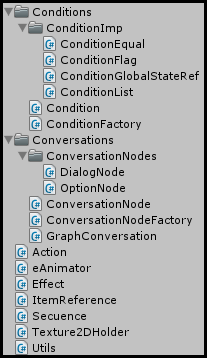
\includegraphics[height=3in]{figures/it1/utilclasses.png}}
	\caption[Clases de Utilidad - Prototipo 1]{Vista de carpeta de las clases de utilidad implementadas en la primera iteración.}
	\label{utilclassesit1}
\end{figure}


La explicación de las clases de utilidad se realiza de forma separada debido a que las clases de utilidad contienen funcionalidad muy diferente entre ellas y no se puede unificar la explicación de las mismas.

\subsection{La clase Texture2DHolder}

La clase Texture2DHolder surge debido a la necesidad de realizar carga de imágenes de manera transparente al usuario, solicitando únicamente al Texture2DHolder que realice la carga de una imagen, a partir de un directorio o unos bytes. Asimismo, esta ayuda a la carga y transformación de imágenes en hilos, ya que Unity3D no permite la carga mediante el método que facilita para carga de recursos, \textit{Resources.Load()}, fuera del bucle principal de ejecución.

Para solventar el problema de la carga paralela de recursos, en lugar de utilizar \textit{Resources.Load()}, se utiliza la librería de sistema, System.IO, utilizando carga de bytes directamente, almacenándolos temporalmente en un \textit{array} de \textit{bytes} dentro de si mismo. para obtener los datos de los ficheros directamente.

Esto causa un pequeño problema a la hora de generar un paquete, y es que, si se desea generar un juego con los recursos incluidos dentro del sistema de empaquetado de Unity, no se podrá acceder a estos recursos, ya que la librería System.IO busca los ficheros en el sistema de ficheros, y \textit{Resources.Load()}, en su lugar, obtiene dichos recursos de los paquetes comprimidos de recursos generados. En la versión final del proyecto, ambos tipos de cargas están permitidos.

Asimismo, Unity no permite generar una \textit{Texture2D}\footnote{Una Texture2D es la clase que se utiliza para guardar texturas bidimensionales en Unity3D, como imágenes, fotografias, o sprites.} si no es en tiempo de ejecución, por lo que, en el momento de la carga sólo se obtienen los bytes, y no es hasta el momento en el que la textura se utiliza por primera vez.

\begin{lstlisting}
public Texture2D LoadTexture(bytes[] fileData)
{
	Texture2D tex = new Texture2D(2, 2,TextureFormat.BGRA32,false);
	tex.LoadImage(fileData);
	return tex;
}
\end{lstlisting}

Tras esto la textura queda guardada y no se vuelve a generar, por lo que se reduce el tiempo de ejecución del programa, a coste de sacrificar memoria. En este caso, como las texturas de los videojuegos generados con eAdventure no ocupan más que el propio juego en sí mismas, se asume que, el coste en memoria de la aplicación no será muy elevado.

\subsection{La interfaz Sequence: Effect, Conversation y Condition})

La interfaz \textit{Sequence} surge de la necesidad de generar una interfaz para interactuar con los efectos y las conversaciones, elementos que son capaces de ejecutarse y realizar tareas que pueden tener alto nivel de complejidad. Esta interfaz, en esencia, provee de un método \textit{public bool execute()}, la cual ejecuta el contenido de si mismas, y devuelve verdadero en caso de que, la secuencia necesite esperar, ya sea por la necesidad de interacción del usuario, o por que un elemento debe ejecutarse un tiempo determinado.

Pese a que la interfaz \textit{Sequence} seguirá existiendo en la versión final del proyecto, se ampliará utilizando la interfaz \textit{Interactuable}, para poder solicitar al usuario que interactúe con algún elemento, ya sea una secuencia, o un elemento interactivo de la escena.

\subsubsection{La clase Effect}

La clase \textit{Effect} es una clase que es híbrida entre Clase de Datos y Clase de Utilidad, pues recibe un \textit{XmlElement} para generarse, y sin embargo aporta funcionalidad por sí misma. Lo que hace dicha clase es: Obtiene un listado de \textit{EffectNode} y de \textit{Condition} y, si existen condiciones, las asigna a cada nodo para que este únicamente se ejecute si cumple las condiciones que permiten su ejecución.

Esta clase contiene dentro de su fichero la clase \textit{EffectNode} el cual, a su vez, contiene cada una de las descripciones de los nodos de una secuencia de efectos. Se implementó en esta iteración del proyecto con una bifurcación, utilizando un \textit{Switch}, en lugar de hacer herencia debido a la cantidad de nodos diferentes, no obstante, en la versión final del proyecto, existen clases para tratar cada uno de los nodos de efecto que componen la secuencia de efectos.

Los \textit{EffectNode} realizan tareas como activar una \textit{Flag}, poner una variable, ejecutar una \textit{Macro}, o ejecutar una condición, por ello tienen dos variables de control que definen su funcionamiento, y una función \textit{execute()} que los pone en funcionamiento. Estas dos variables de control sirven para determinar si dicho nodo sólo se ejecuta una vez, o varias, y para controlar cuántas veces se ha ejecutado ya dicho nodo. Hasta que un nodo no determina que ha completado su ejecución, este no permite que la secuencia se siga ejecutando.

\subsubsection{Las clases GraphConversation y Condition}

Estas clases son las más extensibles de todas las clases que se implementaron en la primera iteración del proyecto. Ambas tienen una factoría para generarse, ya sea \textit{ConditionFactory} y \textit{DialogNodeFactory}, y se generan automáticamente a partir de un \textit{XmlElement}, que contiene la especificación extraída del archivo de especificación del juego.

Por su parte \textit{GraphConversation} solicita a \textit{DialogNodeFactory} un nuevo \textit{DialogNode} por cada uno de sus hijos, y así se genera el diálogo. La “magia” de \textit{DialogNodeFactory} y de \textit{ConditionFactory} es que utilizan \textit{System.Linq}\footnote{El espacio de nombres System.Linq proporciona clases e interfaces que admiten consultas que utilizan Language-integrated query (LINQ)} para examinar el espacio de nombres y obtener de ahí todas las clases que implementan la interfaz \textit{DialogNode} o \textit{Condition}. Esto se realiza de la siguiente manera:
\begin{lstlisting}
types = System.AppDomain.CurrentDomain.GetAssemblies ().SelectMany (s => s.GetTypes ()).Where (p => typeof(ConversationNode).IsAssignableFrom (p)).ToList();

types.Remove(typeof(ConversationNode));
\end{lstlisting}

Y una vez que se ha obtenido la lista de tipos que implementan dicha interfaz, se realiza una búsqueda secuencial, preguntando a cada clase si puede realizar la lectura de dicho \textit{XmlElement}. En caso afirmativo, se le pide que se construya a partir de dicho documento, y la factoría devuelve dicho elemento. Las funciones \textit{canParseType()} y \textit{parse()} están dentro de las inferfaces \textit{DialogNode} y \textit{Condition}. Esto se ve representado en el código que se presenta a continuación:

\begin{lstlisting}
foreach (System.Type t in types)
{
	ConversationNode tmp = (ConversationNode) System.Activator.CreateInstance(t);
	
	if(tmp.canParseType(node.Name))
	{
		tmp.parse(node);
		return tmp;
	}
}
\end{lstlisting}


De esta forma, obtenemos un diseño sencillo y cómodo de extender, pues añadir nuevos tipos de nodo de conversación, o tipos de condiciones es una tarea tan sencilla como generar una nueva clase que implemente esas interfaces, y automáticamente, y sin la necesidad de incluir la existencia de dicha interfaz en la factoría, automáticamente se utiliza.

Si se desea entender o extender el conocimiento de la implementación de estas clases se recomienda mirar el código de estas clases, pues es bastante sencillo y da una visión mucho más clara de su funcionamiento.

\subsection{La clase Action}

Esta clase es tan simple como un efecto con representación. Está compuesta por un Effect que se ejecuta cuando se realiza la acción, una Condition que determina cuando esa acción está disponible, y una serie de recursos que se utilizan para su representación.
La gestión de la visualización de las acciones se realiza en Game, en la funcion OnGUI().

\section{Acerca de los elementos de Adaptación}

El juego Checklist cuenta con un elemento adicional para el jugador, las Adaptation estas no son más que una serie de estados iniciales del juego para que, el juego pueda adaptarse al jugador, ya sea por motivos de accesibilidad o por motivos de nivel.
Las Adaptation se han implementado, pero no existe ningún mecanismo que permite decidir cuál Adaptation se selecciona en cada momento, sino que se selecciona una aleatoriamente al comienzo del juego, y tras esto se trabaja siempre con la misma.


%\chapter{Segunda Iteración: Versión final e Integración}
\label{it2}

Como se explica en el la subsección \ref{metodologiadedesarrollo}, en la que se expone la metodología de desarrollo utilizada para el proyecto, este sufre de tres grandes iteraciones para su completitud. En esta sección se explican los detalles implementados en la segunda iteración, es decir, la generación de un mejor diseño de la aplicación, nuevas interfaces, refactorización de clases y código replicado, así como mejoras gráficas visuales dentro de la aplicación, incluyendo referencias a la sección \ref{primeraiteracion}, explicando los cambios en diseño y comportamiento.

\section{Arquitectura del Proyecto}
\label{it2arquitectura}

La arquitectura del proyecto ha cambiado radicalmente desde la primera iteración, en la que estaba centrada en cómo se debería tratar el documento de especificación de juego, incluido dentro del paquete del juego, en forma de XML para que, cada elemento fuese lo más dinámico posible y sostenible. A su vez, estaba centrada en la clase Game, y existían multitud de clases, llamadas clases de utilidad, que contenían funcionalidad que debía ser accesible a través de una clase controladora de nivel superior.

En esta arquitectura encontramos tres paquetes importantes que engloban la funcionalidad necesaria para la ejecución del proyecto. Están representados en la figura \ref{arquitecturait2} Estos tres paquetes son:

\begin{itemize}
	\item \textbf{Core}: \textit{Core} contiene el núcleo de eAdventure portado a Unity. Este paquete está formado, a su vez, por varios subpaquetes. El primero de ellos es \textit{DataModel}, donde se encuentra todo el modelo de datos portado de eAdventure a Unity, siendo completamente fiel a la implementación realizada en Java, y soportando todas las funcionalidades que se soportaban en dicho editor. El segundo de ellos es \textit{Loader}, donde está contenido el nucleo de lectura y carga del fichero XML de especificación del juego. Este \textit{Loader}, recibe un XML y genera un objeto \textit{AdventureData} que contiene todos los datos del juego. Por último, dentro de \textit{Core} encontramos un paquete \textit{Auxiliar} con clases útiles para este modelo de datos.
	
	\item \textbf{RAGETracker}: que contiene los elementos necesarios para generar un registro de actividad de juego del usuario y comunicarse con RAGE a través de Unity. RAGE se encarga de realizar tareas de evaluación y \textit{Learning Analytics} mediante el análisis de las trazas producidas por el alumno mientras juega. Esto permite al profesor que esté utilizando un juego producido con uAdventure, que se beneficie de las ventajas de RAGE, pudiendo reforzar aquellos alumnos que estén teniendo un desarrollo insuficiente o anormal en el juego.
	
	\item \textbf{Runner}: que se encarga de la transformación desde la especificación una ruta donde hay un juego descomprimido, hasta la generación de un entorno gráfico interactivo que permite al usuario jugar al juego. Contiene 3 subpaquetes que se encargan de diferentes tareas. En primer lugar, el paquete ResourceManager, que se encarga de la carga transparente de recursos, ya sean imágenes, videos, botones, cursores, u otros elementos multimedia. En segundo lugar, el paquete Appearance, que se encarga de mejorar la visualización, mediante diferentes formas de mostrar burbujas de diálogo, o mediante el uso de Shaders. Por último, el paquete \textit{GameLogic and Representation} que se encarga de ejecutar la lógica del juego. Este contiene en su interior una serie de gestores y controladores que son capaces de controlar la ejecución del juego, junto a las secuencias, trayectorias, así como una serie de comportamientos que tomarán lugar dentro de la escena.
\end{itemize}

\begin{figure}[h!]
	\centerline{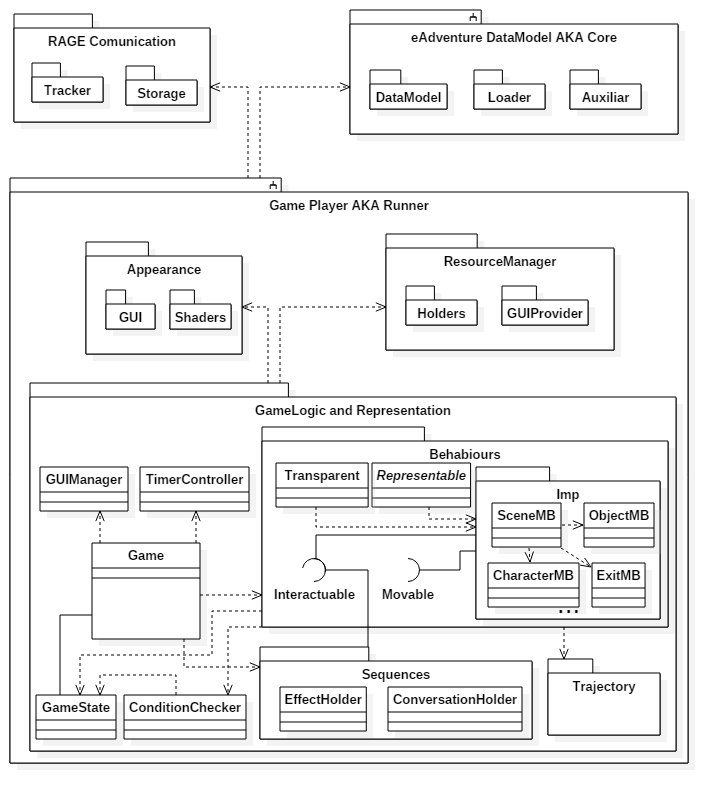
\includegraphics[height=7.5in]{figures/it2/Arquitectura.png}}
	\caption[Arquitectura - Versión Final]{Arquitectura del sistema, a nivel de paquetes de la versión final del proyecto}
	\label{arquitecturait2}
\end{figure}

\newpage

\section{El núcleo de Ejecución: Runner}
\label{runnerit2}

El núcleo de ejecución, también conocido como \textit{Runner}, está dividido en 3 subpaquetes, \textit{Apearance}, encargado de mejorar la representación visual, \textit{ResourceManager}, encargado de realizar la carga transparente de recursos, y \textit{GameLogic}, el cual podría considerarse el núcleo en si mismo, de lógica del juego. Estos tres paquetes surgen de la generalización de elementos que se encontraban, o bien en la antigua clase \textit{Game}, explicada en la sección \ref{gameit1}, o bien en alguna de las clases de utilidad, explicadas en la sección \ref{utilit1}.

De esta manera conseguimos que, la antigua clase controladora del juego \textit{Game}, y las Clases de Utilidad, ahora no tenga que realizar tantas tareas como realizaba anteriormente. En su lugar surgen 5 clases. Estas clases se encargan de hacer transparente la gestión de diversas tareas. Algunas de ellas realizan la gestión de un elemento en concreto, otras controlan la ejecución de otros elementos, y, por último otras se encargan de gestionar el estado del juego.

Estas 5 clases son:
\begin{enumerate}
	\item \textbf{Game}: La clase Game ha sido reducida para encargarse de tres tareas principales: En primer lugar, iniciar la carga y poner en funcionamiento el juego una vez esté cargado. En segundo lugar, controlar la interacción del usuario con los elementos del juego, ya sean elementos con representación, o elementos abstractos como secuencias. Y por último, ser la puerta de enlace que permite elegir qué escena se va a representar.
	
	\item \textbf{GUIManager}: Este gestor se encarga de realizar la gestión de la interfaz que antes se realizaba en \textit{Game}. Permite la emisión de burbujas de diálogo y el control sobre ellas, la posibilidad de mostrar una lista de opciones entre las que el usuario debe seleccionar una respuesta, y por último, la representación de acciones, como botones, y la gestión del menú contextual.
	
	\item \textbf{GameState}: Aunque \textit{GameState} no se considere un \textit{Manager} en si mismo, porque, a diferencia de todos los demás, no es un Singleton, siempre sigue habiendo una única Instancia, pues solo podemos tener un estado de juego, excepto cuando cargamos y guardamos partida. Maneja el estado del juego, que antes se realizaba en \textit{Game}, y facilita funciones para acceder a objetos de la especificación del juego, como \textit{Item} o \textit{NPC}.
	
	\item \textbf{TimerController}: Este gestor que se encarga de controlar los temporizadores que se utilizan en uAdventure para determinadas tareas, como, por ejemplo, hacer que un edificio se queme si no se ha evacuado a tiempo, es, tanto un \textit{Singleton}, como un \textit{MonoBehaviour}, pues necesita de la función \textit{Update()} para controlar que sus temporizadores no hayan saltado. Esta funcionalidad no estaba disponible en la anterior iteración.
	
	\item \textbf{ResourceManager}: este gestor se encarga de facilitar un repositorio transparente a través del cual acceder a los recursos del juego. Añade funcionalidades adicionales que no estaban disponibles anteriormente, como la persistencia en memoria de recursos para agilizar los tiempos de carga, la carga de vídeos, así como la carga de archivos de sonido.
\end{enumerate}

La representación de las clases que se explican en esta sección está disponible en la figura \ref{runnerbigit2}, junto a todas sus funciones. En este diagrama no están representados todos los elementos, pero si aquellos que han surgido de la evolución de las clases que se especificaron al comienzo de la sección. Este diagrama es bastante específico, pues contiene datos acerca de todas las funciones disponibles en cada uno de los elementos.

\newpage

\begin{figure}[h!]
	\centerline{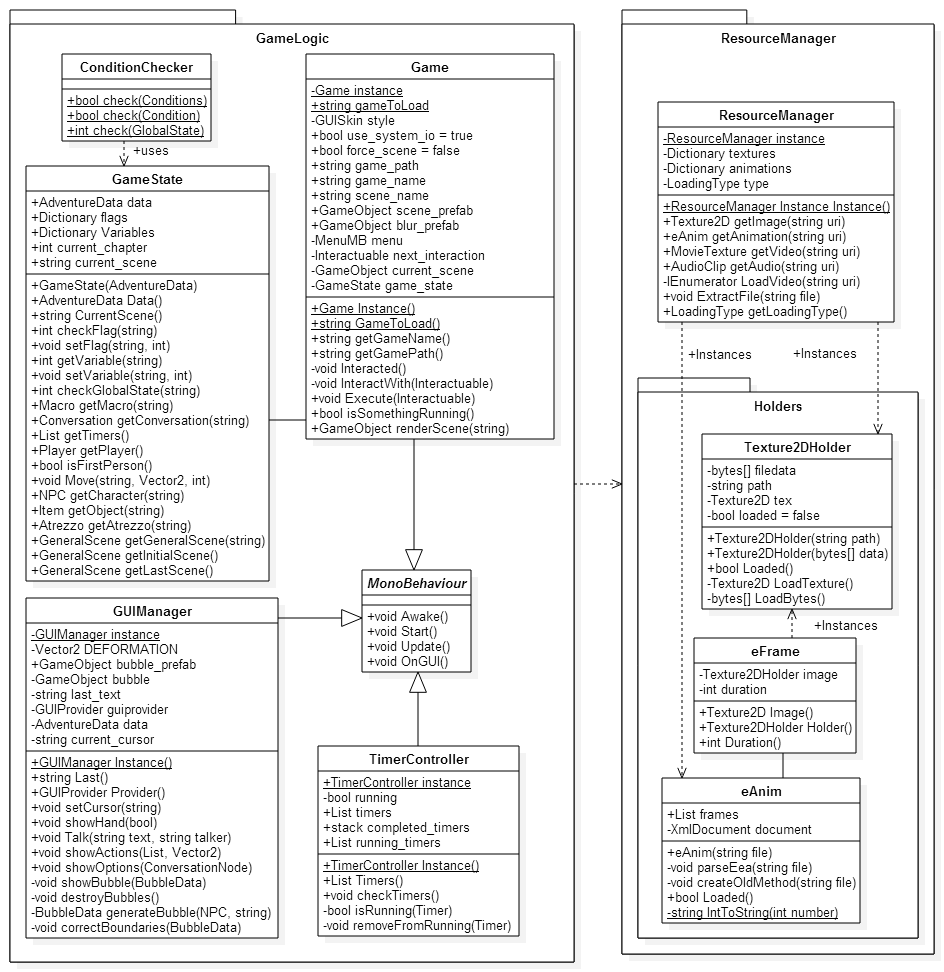
\includegraphics[height=7.5in]{figures/it2/GameLogicBigOnes.png}}
	\caption[GameLogic Grandes Gestores - Versión Final]{Diagrama de clases de los grandes gestores que controlan y proveen contenido para la ejecución del juego.}
	\label{runnerbigit2}
\end{figure}

\newpage

\subsection{El estado del juego: GameState}

Antes de explicar la clase \textit{Game}, es importante explicar la clase que realiza de nexo de unión entre eAdventure y uAdventure, pues esta tiene dos tareas principales: controlar el estado del juego, sus variables, las \textit{Flags} que definen hitos; y la tarea de facilitar el acceso a elementos del juego como los personajes que hay en el capítulo que está siendo jugado en ese momento, como la escena inicial o final de dicho capítulo.

En esencia \textit{GameState} provee un acceso transparente a la especificación del juego en ese momento. Si le pides un personaje, te va a dar la representación de ese personaje en el capítulo que estés jugando. Es importante la relación de asociación direccional que se ve en la figura \ref{gamestateit2} entre \textit{Game} y \textit{GameState}, pues la clase controladora del juego necesita un estado del juego para funcionar, y sin ella, el juego no puede ejecutarse.

\begin{figure}[h!]
	\centerline{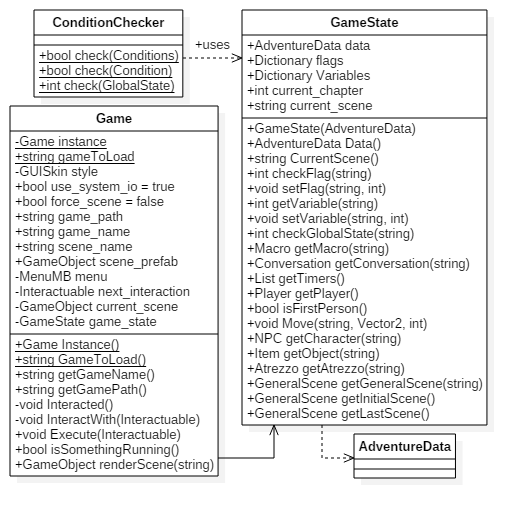
\includegraphics[height=4in]{figures/it2/GameState.png}}
	\caption[GameState - Versión Final]{Diagrama de clases de GameState, junto a Game, ConditionChecker y AdventureData}
	\label{gamestateit2}
\end{figure}

\subsubsection{El validador de Condiciones: ConditionChecker}

Adicionalmente, se muestra en la figura \ref{gamestateit2} a una pequeña clase estática llamada \textit{ConditionChecker}, que se encarga de facilitar la validación de condiciones y estados globales de eAdventure, estas condiciones pueden estar compuestas por multitud de comprobaciones de \textit{Flags} o Variables dentro del \textit{GameState}, por lo que este validador facilita y simplifica mucho el acceso a \textit{GameState}.

\subsection{El Controlador del Juego: Game}
\label{gamesectionit2}

La clase \textit{Game}, ha evolucionado de la clase explicada en la sección \ref{gameit1}. Como se ha mencionado multitud de veces a lo largo de la sección \ref{arquitecturait2}, esta clase \textit{Game} ha evolucionado para delegar comportamientos en los 5 grandes gestores. Sin embargo, la funcionalidad que \textit{Game} aporta en el ciclo de vida y ejecución del juego sigue siendo de vital importancia.

Esta clase \textit{Game} ahora se encarga de 3 tareas: iniciar la carga y poner en funcionamiento el juego una vez esté cargado; controlar la interacción del usuario con los elementos del juego, así como con efectos y conversaciones; y ser la puerta de enlace que permite elegir qué escena se va a representar. No obstante estas tres tareas son vitales, pues en esencia, un juego sólo se puede jugar si se trata esta funcionalidad.

Como la clase \textit{Game} es la puerta de enlace que transforma de una clase \textit{AventureData} a algo jugable, junto a la explicación de \textit{Game}, como subapartados, se presentarán los comportamientos encargados de enrolarse como los diferentes elementos que forman las escenas de eAdventure.

Uno de los cambios más notorios en todo el núcleo de representación es la desaparición de las Clases de Datos explicadas en la sección \ref{dataclassesit1}. Esto es debido a la incorporación del modelo de datos original portado directamente de eAdventure.

En la figura \ref{gameit2} se muestra un diagrama de clases que explica las relaciones de las clases que participan en esta representación del juego. Aunque \textit{SceneMB} tenga una relación de dependencia con \textit{Game}, la escena únicamente necesita acceder a \textit{GameState}, para obtener las especificaciones de los elementos que va a instanciar. \textit{SceneMB} a su vez mantiene relación de dependencia con \textit{PlayerMB}, \textit{CharacterMB}, \textit{ObjectMB}, etc... debido a que \textit{SceneMB} instancia todas estas clases como hijas suyas.


\begin{figure}[h!]
	\centerline{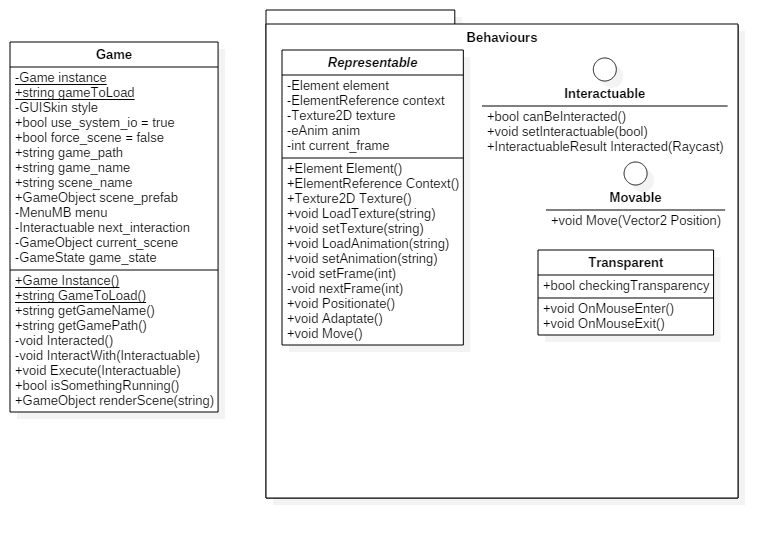
\includegraphics[height=7.2in]{figures/it2/Game.png}}
	\caption[Game - Versión Final]{Diagrama de clases de Game, con todo el nucleo de representación}
	\label{gameit2}
\end{figure}

\subsubsection{Representable, Interactuable, Movable y Transparent}

Este grupo está compuesto por dos clases y dos interfaces, y permiten a la implementación de los comportamientos facilitar la definición de lo que pueden y no pueden hacer. Las dos interfaces son Interactuable y Movable. Tras esto encontramos Representable como clase abstracta que ayuda a la representación de todos los elementos que utilizan recursos, facilita la relación con el \textit{ResourceManager}, y, al extender la clase \textit{MonoBehaviour}, permite a todos los elementos que la extienden ser componentes a su vez. Por ultimo tenemos la clase \textit{Transparent} que, facilita la interacción con elementos que, por motivos de representación en su imagen, no ocupan toda la imagen, teniendo transparencia.

En primer lugar, hablando de \textit{Interactuable}, es la interfaz que permite a \textit{Game} la interacción entre el usuario y los elementos de la escena. \textit{Game}, cuando detecta una pulsación de ratón, lanza un rayo desde dicha posición, en dirección en la que mira la cámara, obtiene una lista de objetos, y, si implementan la interfaz \textit{Interactuable}, les notifica que se ha realizado una interacción con ellos. Estos tienen tres opciones que responder: que no van a hacer nada con la interacción, que hacen algo con ella, o que hacen algo y además esperan más por parte del usuario. En el momento en que \textit{Game} detecta alguna que hace algo, deja de notificar a los demás.

En segundo lugar, hablando de \textit{Movable} es una interfaz sencilla que deben implementar todos aquellos elementos que deseen moverse. Y que únicamente tiene un método \textit{Move()}

En tercer lugar, hablando de \textit{Representable}, encontramos la clase abstracta más compleja, pues permite a los elementos anteriormente citados representarse. Por si misma no realiza ninguna tarea, necesita que la clase que la extienda le indique lo que necesita. Por ejemplo, un objeto de Atrezzo, en su función \textit{Start()} realiza lo siguiente:

\begin{lstlisting}
void Start()
{
	base.Start ();
	base.setTexture(Atrezzo.RESOURCE_TYPE_IMAGE);
	base.Positionate ();
}
\end{lstlisting}

Además de esto, \textit{Representable}, se encarga de transformar esa línea de especificación de recurso \textit{Atrezzo.RESOURCE\_TYPE\_IMAGE} en una \textit{Texture2D} mediante el uso del \textit{ResourceManager}. Asimismo, esta clase \textit{Representable} tiene también facilidades para el uso de animaciones y su actualización en fotogramas.

Finalmente, hablando de la clase \textit{Transparent} es una componente que se añade a los objetos de la escena, y tiene una relación de dependencia con ellos, ya que, sin esta clase, nunca se habilitarían dichos objetos para permitir la interacción con ellos. En \textit{Transparent} se analizan los píxeles de la textura activa en \textit{Representable}, y, si el píxel sobre el cual se tiene el ratón no es transparente, es decir, su componente \textit{Alpha} de color es mayor que 0, se accede a \textit{Interactuable} y se establece como que se puede realizar interacción con dicho elemento.

Estos cuatro elementos de los que se componen los objetos de la escena están representados en la figura \ref{behavioursit2}, con sus relaciones.

\begin{figure}[h!]
	\centerline{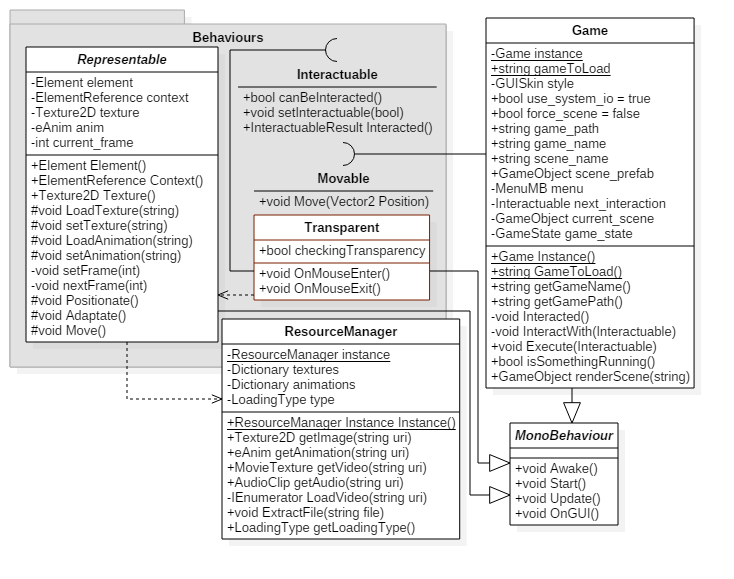
\includegraphics[height=4in]{figures/it2/Behaviours.png}}
	\caption[Representable, Interactuable, Movable y Transparent - Versión Final]{Diagrama de clases de Representable, Interactuable, Movable y Transparent}
	\label{behavioursit2}
\end{figure}

\newpage

\subsection{La escena y sus elementos}

La escena de eAdventure, además de poder ser de multitud de tipos diferentes, está llena de elementos, algunos de ellos que están "vivos", otros que permiten interacción, y otros que únicamente son elementos que mejoran la representación visual. En conjunto, todos estos elementos permiten representar lo que se desee dentro de un escenario. Los elementos que se presentan en esta sección evolucionan de los explicados en la sección \ref{behavioursit1}.

En esta sección se remarcan las diferencias entre las clases de comportamiento presentadas en la sección \ref{behavioursit1} y las actuales, especificando cómo han evolucionado estas. En esencia, su funcionalidad se ha mantenido, o delegado en otras clases, así como han ganado funcionalidad extraída de la clase \textit{Game}. Esto es debido a que siguen siendo los mismos elementos que conforman la escena.

Otro detalle es, para diferenciar más fácilmente entre las clases del modelo de datos y los comportamientos, se les han añadido las siglas MB de \textit{MonoBehaviour}, que identifican que son comportamientos y no clases de datos.

\subsubsection{Detalles de la escena: SceneMB}
\label{scene}

La escena ha sido refactorizada y ampliada para incluir más funcionalidad y facilitar el uso de otra. Detalles de esto se puede encontrar en la figura \ref{gameit2}.

En primer lugar, ahora la escena da soporte a vídeos, aunque estos vídeos han de estar en formato OGV\footnote{El formato OGV es el contenedor de archivo de vídeo que utiliza el códec libre de video Theora.}. Se ha realizado una investigación para determinar si es posible realizar una conversión del formato de los vídeos y su explicación se encuentra en la sección dedicada a la tercera iteración del proyecto.

En segundo lugar, la escena ha simplificado la instanciación de sus elementos, e implementa dos métodos para dicha tarea, los cuales son:

\begin{lstlisting}
private void instanceElement<T>(ElementReference context) where T : Element
private void instanceRectangle<T>(Rectangle context) where T : Rectangle
\end{lstlisting}

Estas funciones, pese a ser funciones tipadas, tienen la peculiaridad de delimitar el tipo de clases que admiten. Esto se consigue utilizando \textit{where T : Interface}.

En tercer lugar, como ahora el juego tiene soporte a juegos en tercera persona, en los que el jugador forma parte de la escena, esta ahora puede contener trayectorias para que el jugador se pueda mover sobre ellas. El cálculo de estas trayectorias fue una de las tareas más complejas de implementar, y se explica en la sección \ref{trajectoryit2}.

Por último, ahora la escena gestiona la interacción que se realice sobre ella, aunque es diferente dependiendo de qué tipo de escena se esté mostrando:
\begin{itemize}
	\item \textbf{Scene}: Si la escena es una escena normal, y además el juego es en tercera persona, se busca el punto que sea más cercano a la trayectoria, se calcula una ruta para que el jugador llegue a ese punto, y se le indica al jugador que inicie el movimiento dada dicha ruta.
	
	\item \textbf{SlideScene}: Si la escena contiene diapositivas, pasaremos a la siguiente diapositiva. Si por el contrario ya no quedan, se continuará a la escena que la siga, ya sea la anterior o una nueva.
	
	\item \textbf{VideoScene}: Si se recibe una interacción, se para el vídeo, y se continúa cargando la siguiente escena igual que en una \textit{SlideScene}.
\end{itemize}

\subsubsection{Los objetos del juego: ObjectMB}
\label{itemsit2}

Con respecto a lo explicado en la sección \ref{objectexitactiveareait1} acerca de la antigua clase \textit{eObject}, esta ha sufrido una evolución. Se ha simplificado mucho gracias al uso de \textit{Representable}, \textit{Interactuable} y \textit{Transparent}. Ahora únicamente reacciona si la componente \textit{Transparent} se lo permite, y gracias a \textit{Representable} y al \textit{ResourceManager} es mucho más sencillo cambiar entre la textura normal y la textura activa, que se debe mostrar cuando el ratón pasa por encima el objeto.

Por otra parte, los objetos implementan una nueva funcionalidad, que les permite ser arrastrados en vez de generar un menú contextual cuando se interactúa con ellos. La especificación de cuándo esto debe suceder se encuentra en la propia especificación del \textit{Item} que se está representando. Se remarca lo descrito en la sección \ref{gamesectionit2} acerca de la desaparición de las clases de datos descritas en la sección \ref{dataclassesit1}, y la sustitución de las mismas por el modelo de datos de eAdventure.

\subsubsection{Las deformables ActiveAreasMB}
\label{activeareasectionit2}

Como se ha mencionado en secciones anteriores, en la versión final, las \textit{ActiveAreas} adquieren la capacidad de deformarse. Esto se consigue gracias a la utilización del Área de Influencia facilitado en la especificación del \textit{ActiveArea}.

En la función \textit{adaptate()}, una \textit{ActiveArea} se encarga de leer esta \textit{InfluenceArea}, y transformar estos puntos, que se encuentran en coordenadas relativas a la escena, a puntos colocados alrededor del centro de ellos. Tras esto se utiliza la libreria \textit{LibTessDotNet} que genera una lista de triángulos a partir de esos puntos.

Una vez se obtienen los puntos y la lista de triángulos, se genera una nueva malla tridimensional estableciendo los vértices en dicha malla, y los triángulos en forma de referencias a los índices de la lista de vértices. Una vez generada dicha malla, se intercambia la \textit{SharedMesh}\footnote{La SharedMesh es una componente de los objetos tridimensionales de Unity3D que contiene la malla tridimensional que lo representa.} por la nueva malla, consiguiendo como resultado un objeto tridimensional con la forma deseada.

Finalmente, este elemento de la escena, como muchos otros elementos interactivos, tienen una componente \textit{AutoGlower}, la cual se explica en la sección \ref{apearanceseccionit2}, que hace que brillen durante un instante cada intervalo regular de tiempo.

Esto se ve representado en la figura \ref{activeareasit2}. Las figuras blancas son las áreas de influencia que dan forma a dichas areas activas. Estas capturas han sido obtenidas del juego utilizado para formar acerca de los primeros auxilios, desarrollado por Catedu.

\begin{figure}[h!]
	\centerline{\includegraphics[height=3in]{figures/it2/Apearance/ActiveAreas.png}}
	\caption[ActiveAreas - Versión Final]{Representación de las ActiveAreas en el videojuego FirstAid}
	\label{activeareasit2}
\end{figure}

\subsubsection{Las clases vivas: PlayerMB y CharacterMB}
\label{playerit2}

De las clases mostradas anteriormente, existen dos clases que implementan la interfaz \textit{Movable}, pues necesitan moverse por la escena. Estas son \textit{CharacterMB} y \textit{PlayerMB}.

En esencia estos dos elementos de la escena son iguales, salvo por la peculiaridad de que \textit{CharacterMB} permite interactúar con el, y realizar acciones que requieran la interacción con ella. Como dicha interacción es trivial, únicamente se explica la parte relacionada con la gestión del movimiento y animaciones.

En primer lugar, cuando en una de estas clases es invocada la función \textit{Move()}, se genera una cola de puntos a los que se debe ir. Tras esto se establece el primer nodo de la cola como nodo destino, y, dependiendo de la dirección hacia la que se deba desplazar para alcanzar dicho nodo, se muestra una animación u otra. Cuando el movimiento se completa y se alcanza el nodo destino, el siguiente nodo de la cola pasa a ser el nodo objetivo, y se realiza el mismo proceso hasta completar la cola de nodos. 

En segundo lugar, cuando una de estas es llamada a hablar, si esta tiene animaciones para el diálogo, se activan mientras la burbuja de diálogo siga activa.

\subsubsection{Las trayectorias: TrayectoryHandler}
\label{trajectoryit2}

La gestión de las trayectorias dentro de la escena es una de las labores más complejas de realizar, pues, en general, los algoritmos de búsqueda de rutas suelen ser algoritmos complejos, y la interacción con una trayectoria, que es algo simbólico, una lista de puntos en el espacio, unidos por líneas, es una tarea compleja.

Por ello, para la gestión de trayectorias, se han implementado 3 clases necesarias para funcionalidades concretas:

\begin{enumerate}
	\item \textbf{TrajectoryHandler}: esta clase es la encargada de proveer el manejo de una \textit{Trajectory} de eAdventure. Se genera a partir de una de estas, y facilita funciones capaces de generar rutas entre puntos que se encuentren en dichas trayectorias.
	
	\item \textbf{LineHandler}: esta clase se encarga de la gestión de una Línea de trayectoria. Está compuesta por dos nodos y la línea que los une. Tiene funciones para determinar que líneas son vecinas de esta línea, cuales son los puntos de contacto a partir de otro punto, o si saber si un punto está contenido en dicha línea.
	
	\item \textbf{MathFunction}: esta clase, dados dos puntos de una recta, mediante el uso de funciones matemáticas, es capaz de generar un valor Y para una X dada, o un valor X para una Y dada, así como es capaz de generar puntos de contacto a partir de otro punto.
\end{enumerate}

El tratamiento de trayectorias comienza con la generación de un \textit{TrajectoryHandler}, este analiza dicha trayectoria, y para cada lado de esta genera un \textit{LineHandler}. Una vez que todos han sido generado, se llama a la función \textit{UpdateNeighbors()} que recorre esta lista de líneas y, si dos líneas contienen extremos comunes, se determina que estas son vecinas.

Las líneas, cuando son generadas, utilizan sus dos puntos para generar una \textit{MathFunction} que les ayudará a generar y a determinar puntos que estén en su línea.

Lo complejo del tratamiento de trayectorias llega con el cálculo de rutas. Para ello se ha implementado una variante del algoritmo de Dijkstra para hallar caminos mínimos en grafos no direccionales con coste. La diferencia es que, debido a que en la ruta el nodo inicial y el nodo final no forman parte de la trayectoria en si misma, sino que son nodos nuevos que se generan en tiempo de ejecución, y únicamente se identifica en qué líneas de trayectoria están contenidos dichos puntos.

Tras esto se identifica que líneas contienen el punto de origen y el punto destino, y con esto se realiza el algoritmo de marcado de Dijkstra pero únicamente utilizando las líneas, sin los nodos. Y finalmente se ejecuta la función \textit{reach()} que prepara el lanzamiento de la función recursiva de mismo nombre encargada de recorrer el grafo siguiendo la especificación del algoritmo de Djikstra.

No obstante, el funcionamiento de este algoritmo no es tan bueno como se desearía, pues le falta incluir la distancia que hay entre el punto de origen o destino, y el nodo inicial elegido de la línea de origen y destino. Asimismo, se pueden dar resultados no optimos. Como trabajo futuro se plantea implementar el algoritmo de Djikstra con nodos, e incluir los nodos origen y destino en la trayectoria.

\begin{figure}[h!]
	\centerline{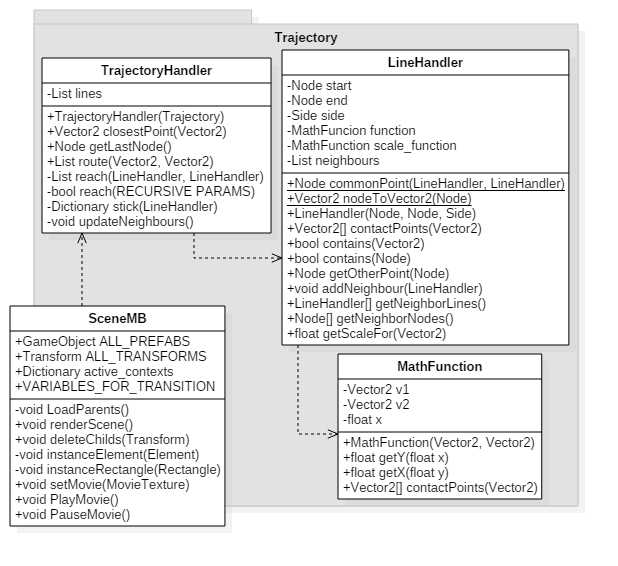
\includegraphics[height=3.7in]{figures/it2/TrajectoryHandler.png}}
	\caption[TrajectoryHandler - Versión Final]{Diagrama de clases de las trayectorias, junto a LineHandler y MathFunction}
	\label{trajectoryfigit2}
\end{figure}

\subsection{Las secuencias: Effect y GraphConversation}
\label{sequencesit2}

La implementación de las secuencias, visible en la figura \ref{sequencesfigit2}, tanto de efectos, como de conversación cambió mucho desde la primera iteración hasta la segunda iteración. En esencia, se han eliminado las factorías de efectos, pues estas ya no necesitan ser autogeneradas a partir del fichero de especificación en XML, pues el paquete \textit{Loader} del modelo de eAdventure ya se encarga de realizar dicha lectura.

Sin embargo, siguen manteniendo la esencia, y no se ha implementado ningún \textit{SequenceManager} que se encargue de ejecutar las secuencias. En su lugar, siguen siendo autoejecutables, siendo más sencillo de recordar estados si la escena se para en la mitad de su ejecución y a su vez contiene llamadas a secuencias dentro de si mismas.

Mas allá de esto, el esfuerzo se realizó añadiendo la mayor parte de efectos disponibles en eAdventure, y únicamente dejando unos pocos por implementar, y por otra parte, haciendo funcionar los \textit{Holders}, con las clases del modelo de datos de eAdventure.

\begin{figure}[h!]
	\centerline{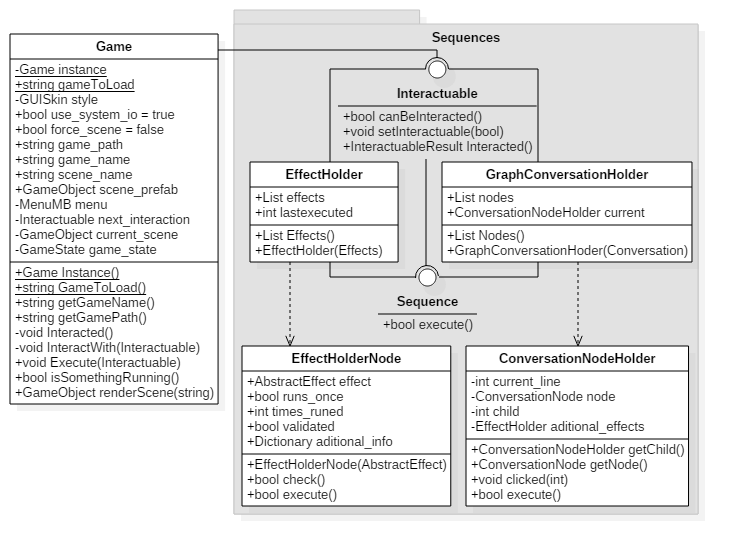
\includegraphics[height=3.7in]{figures/it2/Sequences.png}}
	\caption[Sequences - Versión Final]{Diagrama de clases de las Secuencias, mostrando tanto EffectHolder como GraphConversationHolder}
	\label{sequencesfigit2}
\end{figure}

\subsection{El controlador de los temporizadores: TimerController}
\label{timercontrollersecit2}

El controlador de los temporizadores es una clase nueva que no existía en la anterior iteración. Esta clase comportamiento se añade como componente a la cámara y se encarga, mientras está contando, de controlar los \textit{Timers} que el juego necesita para su ejecución.

Para manejar los temporizadores se ha implementado un enumerado llamado \textit{TimerType} que establece el tipo de temporizador que se está tratando, y una clase llamada \textit{TimerState} que únicamente sirve para almacenar datos acerca de los temporizadores que se encuentran en ejecución.

Este controlador tiene además la opción de parar su ejecución para que, si el juego se encuentra parado esperando a que el jugador interactúe en una secuencia, no salten temporizadores en mitad de dicha secuencia. 

Para gestionar estos temporizadores se tienen tres listas:  una lista con todos los temporizadores de dicho capítulo, una lista con los temporizadores que están ejecutándose, y por último una cola con los que ya se han completado.

Se aprovecha de la función \textit{Update()} de \textit{MonoBehaviour} para controlar el paso del tiempo en los mismos, así como detectar qué temporizadores cumplen las condiciones para ejecutarse, y cuáles de los que se encuentran en ejecución ya no deberían estar ejecutándose.

\begin{figure}[h!]
	\centerline{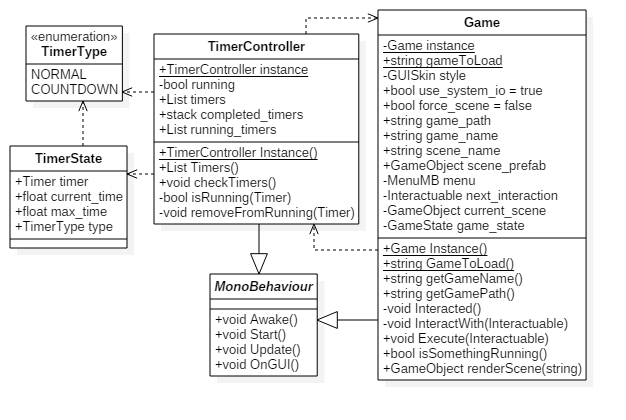
\includegraphics[height=4in]{figures/it2/TimerController.png}}
	\caption[TimerController - Versión Final]{Diagrama de clases de TimerController, incluyendo las clases y enumerados para su funcionamiento.}
	\label{timercontrollerit2}
\end{figure}

la figura \ref{timercontrollerit2} muestra el diagrama de clases de lo descrito anteriormente. En este diagrama se ve como \textit{Game} establece los \textit{Timers} que deben ser controlados al inicio de cada capítulo, y \textit{TimerController} únicamente los gestiona. Cuando alguno de estos \textit{Timers} se completa, \textit{TimerController} le dice a \textit{Game} que ejecute los efectos de dicho temporizador.

\newpage

\subsection{El gestor de interfaz: GUIManager}
\label{guimanagersectionit2}

Como se explica en la sección superior a esta subsección, existe una clase gestora que se encarga de manejar la interfaz en su totalidad de forma transparente. Facilita una serie de funciones que permiten, de forma sencilla, mostrar burbujas de diálogo, cambiar el cursor, mostrar un menú contextual de acciones, o un menú de opciones.

Este gestor surge de la reducción de contenido de \textit{Game}, que antes realizaba estas tareas, y fue relevada de su función debido a que dicha clase comenzaba a tener una dimensión demasiado elevada. La figura \ref{guimanagerit2} muestra el diagrama de clases de la clase \textit{GUIManager} junto al paquete \textit{Apearance}, el paquete \textit{GUIProvider} que contiene todo lo necesario para acceder al \textit{ResourceManager} de forma automática y transparente, así como la carga de recursos por defecto y la gestión de nombres a constantes y viceversa, y el paquete \textit{Menu}, que contiene una serie de clases para la representación y animación del Menú.

Este gestor hereda de \textit{MonoBehaviour}, por lo que es asignado como componente de un elemento dentro de la escena. En este caso se asigna a un objeto \textit{Canvas}, que permite la representación de elementos de interfaz. 

El ciclo de vida de \textit{GUIManager} comienza cuando despierta la escena. En este momento se establece como instancia a si mismo. Tras esto, cuando \textit{Game} ya ha cargado el juego, y se ejecuta la función \textit{Start()}, este provee al \textit{GUIProvider} de los datos del juego en forma de un \textit{AdventureData}. Este se prepara y carga los recursos que deba cargar, y tras esto, el \textit{GUIManager} se queda en espera hasta que el juego necesite mostrar al usuario algo.

Una vez que el \textit{GUIManager} se encuentra en espera, facilita una serie de funciones útiles para representar cosas al usuario, estas son:
\begin{itemize}
	\item \textbf{Talk(string line, string talker)}: Esta función permite al sistema que los personajes hablen. Esto se ha implementado mediante el uso de burbujas.
	
	\item \textbf{showActions(List<Actions>, Vector2 position)}: Esta función pone en ejecución al menú contextual, y hace que se muestre con las acciones especificadas en una posición.
	
	\item \textbf{showOptions(ConversationNode)}: Esta función permite mostrar un listado de opciones de texto que el usuario debe elegir. Adicionalmente, el fondo se emborrona y se muestra el texto de la última pregunta.
	
\end{itemize}


\begin{figure}[h!]
	\centerline{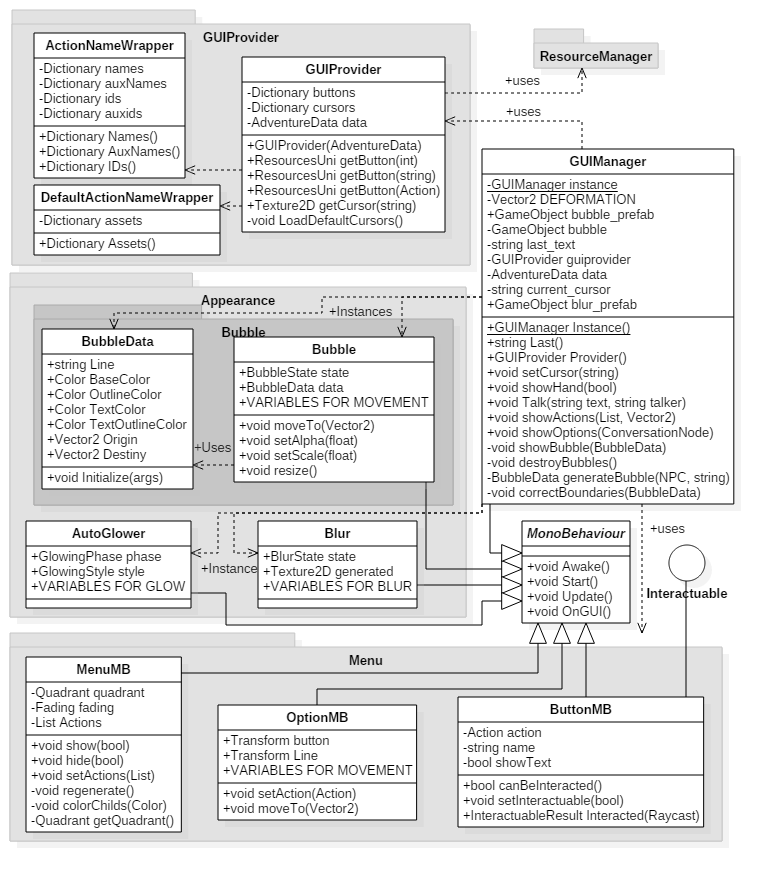
\includegraphics[height=7.5in]{figures/it2/GUIManager.png}}
	\caption[GameLogic Grandes Gestores - Versión Final]{Diagrama de clases de los grandes gestores que controlan y proveen contenido para la ejecución del juego.}
	\label{guimanagerit2}
\end{figure}

\newpage

\subsubsection{Proveedor de recursos de GUI: GUIProvider}

La interfaz es una capa de la vista que necesita representación, y por ello, necesita acceder a recursos para poder representarse. Sin embargo, nuestro gestor de \textit{GUI} no usa directamente al \textit{ResourceManager}, sino que utiliza una clase intermedia para acceder a los recursos, esta clase es \textit{GUIProvider}, y se encarga de, facilitar el acceso a texturas que tengan una funcionalidad concreta. Es decir, por ejemplo, obtener la textura que representa a una acción, o el cursor que se debe mostrar para un determinado elemento. \textit{GUIProvider} se encarga de proveer los recursos apropiados.

Además de esto, eAdventure sigue una jerarquía a la hora de definir recursos para la interfaz, esta es la siguiente:

\begin{enumerate}
	\item Se cargan los recursos por defecto. Estos recursos están repartidos en dos directorios, el primero es la carpeta "~/gui/hud/contextual/" donde se encuentran los botones que representan los distintos tipos de acciones y que se obtienen utilizando la clase \textit{DefaultActionNameWrapper}. El segundo el la carpeta "~/gui/cursors/" donde se encuentran los cursores del juego, y que se obtienen utilizando la clase \textit{ActionNameWrapper}. Estas dos clases \textit{Wrapper} se encargan de transformar de Acción, o identificador de Acción a nombre, y viceversa.
	
	\item Se cargan los recursos especificados en la base del archivo "descriptor.xml". Tras la lectura de dicho archivo en \textit{Loader}, estos se encuentran en el objeto de datos \textit{AdventureData} que gestiona \textit{GameState}. Estos también se asignan utilizando los \textit{Wrappers} anteriormente especificados, y, sustituyen a los botones y cursores cargados en el apartado anterior con los que se hayan en esta especificación.
	
	\item Por último puede ocurrir una situación anómala, y es que un elemento tenga una acción personalizada en su interior. En este caso, y excepcionalmente, es el propio botón del menú el que se encarga de solicitar al \textit{ResourceManager} dichos recursos.
	
\end{enumerate}

\begin{figure}[h!]
	\centerline{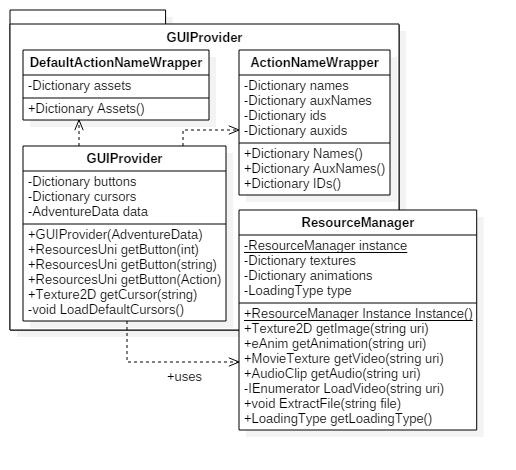
\includegraphics[height=3.5in]{figures/it2/GUIProvider.png}}
	\caption[GUIProvider - Versión Final]{Diagrama de clases de GUIProvider, junto con ResourceManager.}
	\label{guiproviderit2}
\end{figure}

Las clases que participan en este proceso están representadas en la figura \ref{guiproviderit2}. En esta figura, aunque \textit{ResourceManager} esté sobrepuesto al paquete \textit{GUIProvider}, esto es debido a reducir el tamaño del diagrama, realmente este no forma parte de dicho paquete.

\subsubsection{Las burbujas de diálogo: Bubble}

La representación de diálogos en un juego de aventuras es una tarea necesaria, pues los personajes necesitan hablar para compartir información entre ellos. La manera de representar estos diálogos en uAdventure es la misma que se decidió utilizar en eAdventure: Las burbujas de diálogo, o bocadillos de diálogo. Sin embargo, estas burbujas han evolucionado en su representación, realizando una pequeña animación a la hora de ser invocadas, y a la hora de desaparecer.

\begin{figure}[h!]
	\centerline{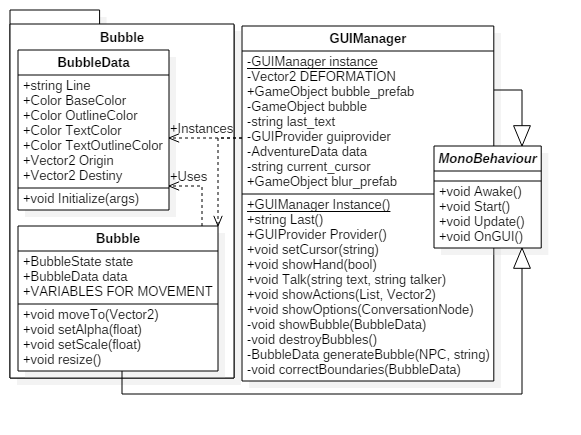
\includegraphics[height=3.5in]{figures/it2/Bubble.png}}
	\caption[Bubble - Versión Final]{Diagrama de clases de Bubble, junto con GUIManager y MonoBehaviour.}
	\label{bubbleit2}
\end{figure}

El proceso de mostrar una burbuja de diálogo comienza en \textit{GUIManager} y es el siguiente: En primer lugar, se identifica si el que habla es el jugador o un personaje, y si es el jugador, se distingue si se trata de un juego en primera persona o un juego en el que el jugador tenga representación en el juego. Una vez se ha determinado quién habla, se obtienen los datos del hablante y se genera una \textit{BubbleData} con dichos datos, decorándola y estableciendo su trayectoria. Este \textit{BubbleData} se pasa a través de una serie de deformaciones que adaptan dichas trayectorias a la pantalla para que no se salga de la misma, y para que se coloque correctamente independientemente de la resolución de la misma. Tras esto se instancia una nueva burbuja en la escena y se delega en ella.

La burbuja, en su función \textit{Start()}, establece su texto en la representación, se prepara para moverse, y se prepara para empezar a mostrarse, pues al principio es transparente. Poco a poco esta se va moviendo y haciéndose visible en su función \textit{FixedUpdate()}, y cuando termina, se queda quieta. Cuando es necesario que la burbuja desaparezca, se ejecuta la función \textit{destroy()} que la hace desaparecer poco a poco, haciéndose más pequeña y transparente.

\subsubsection{Elementos de mejora visual: Apearance}
\label{apearanceseccionit2}

Existen dos clases que, para mejorar la representación visual del juego, se han desarrollado en el proyecto. Cómo se explicó en el apartado \ref{eandroidmokap} del estado del arte, y visible en la figura \ref{eandroidlupa}, el proyecto eAdventure Android utilizaba mecanismos específicos para ayudar al usuario a encontrar elementos en un entorno táctil. En este proyecto, para ayudar al usuario a encontrar estos elementos, se realiza un brillo de los mismos.

La clase componente \textit{AutoGlower} se encarga de realizar este brillo sobre los objetos que la contengan. Tiene varios modos, como simplemente hacer un flash, o aparecerse y desvanecerse y hacer un flash. Este \textit{AutoGlower} utiliza un \textit{Shader} que genera dicho flash y que es parametrizable para establecer tanto la posición del brillo, su color y su anchura. Este efecto es visible en las figuras \ref{autoglow1it2} y \ref{autoglow2it2};

\begin{figure}[h!]
	\centerline{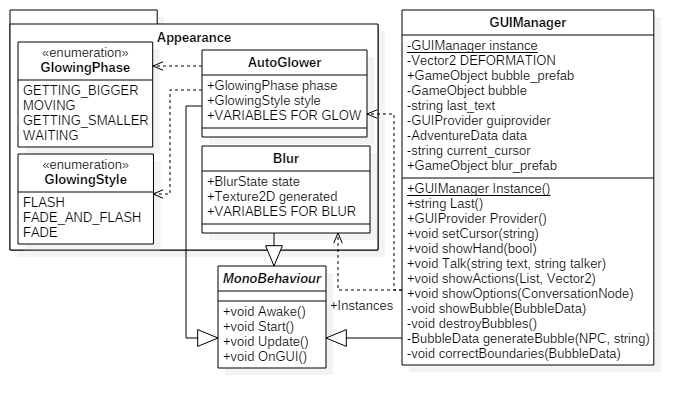
\includegraphics[height=3.5in]{figures/it2/Apearance.png}}
	\caption[Apearance - Versión Final]{Diagrama de clases de Apearance, sin incluir Bubble.}
	\label{apearanceit2}
\end{figure}

Por último, tenemos a la clase \textit{Blur}, que, al igual que la anterior utiliza un \textit{Shader} para conseguir su efecto visual. En este caso, \textit{Blur} lo que hace es volver borroso lo que hay detrás de ella. Es utilizada para generar un cuadrado borroso sobre el cual presentar las distintas opciones disponibles en la lista de opciones de una conversación. Este efecto se puede ver en la figura \ref{blurit2}.

\begin{figure}[h!]
	\centerline{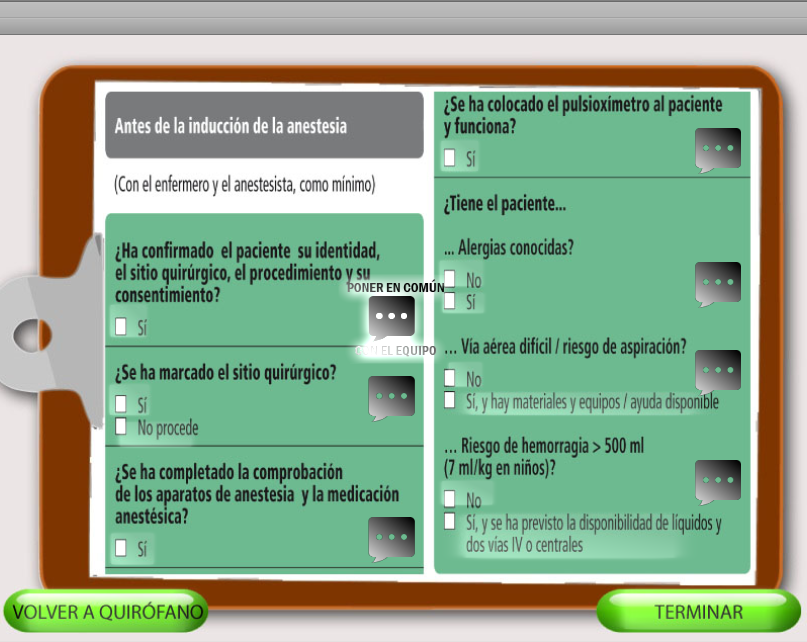
\includegraphics[width=4.3in]{figures/it2/apearance/checklist.png}}
	\caption[Apearance - Versión Final]{Diagrama de clases de Apearance, sin incluir Bubble.}
	\label{autoglow1it2}
\end{figure}

\begin{figure}[h!]
	\centerline{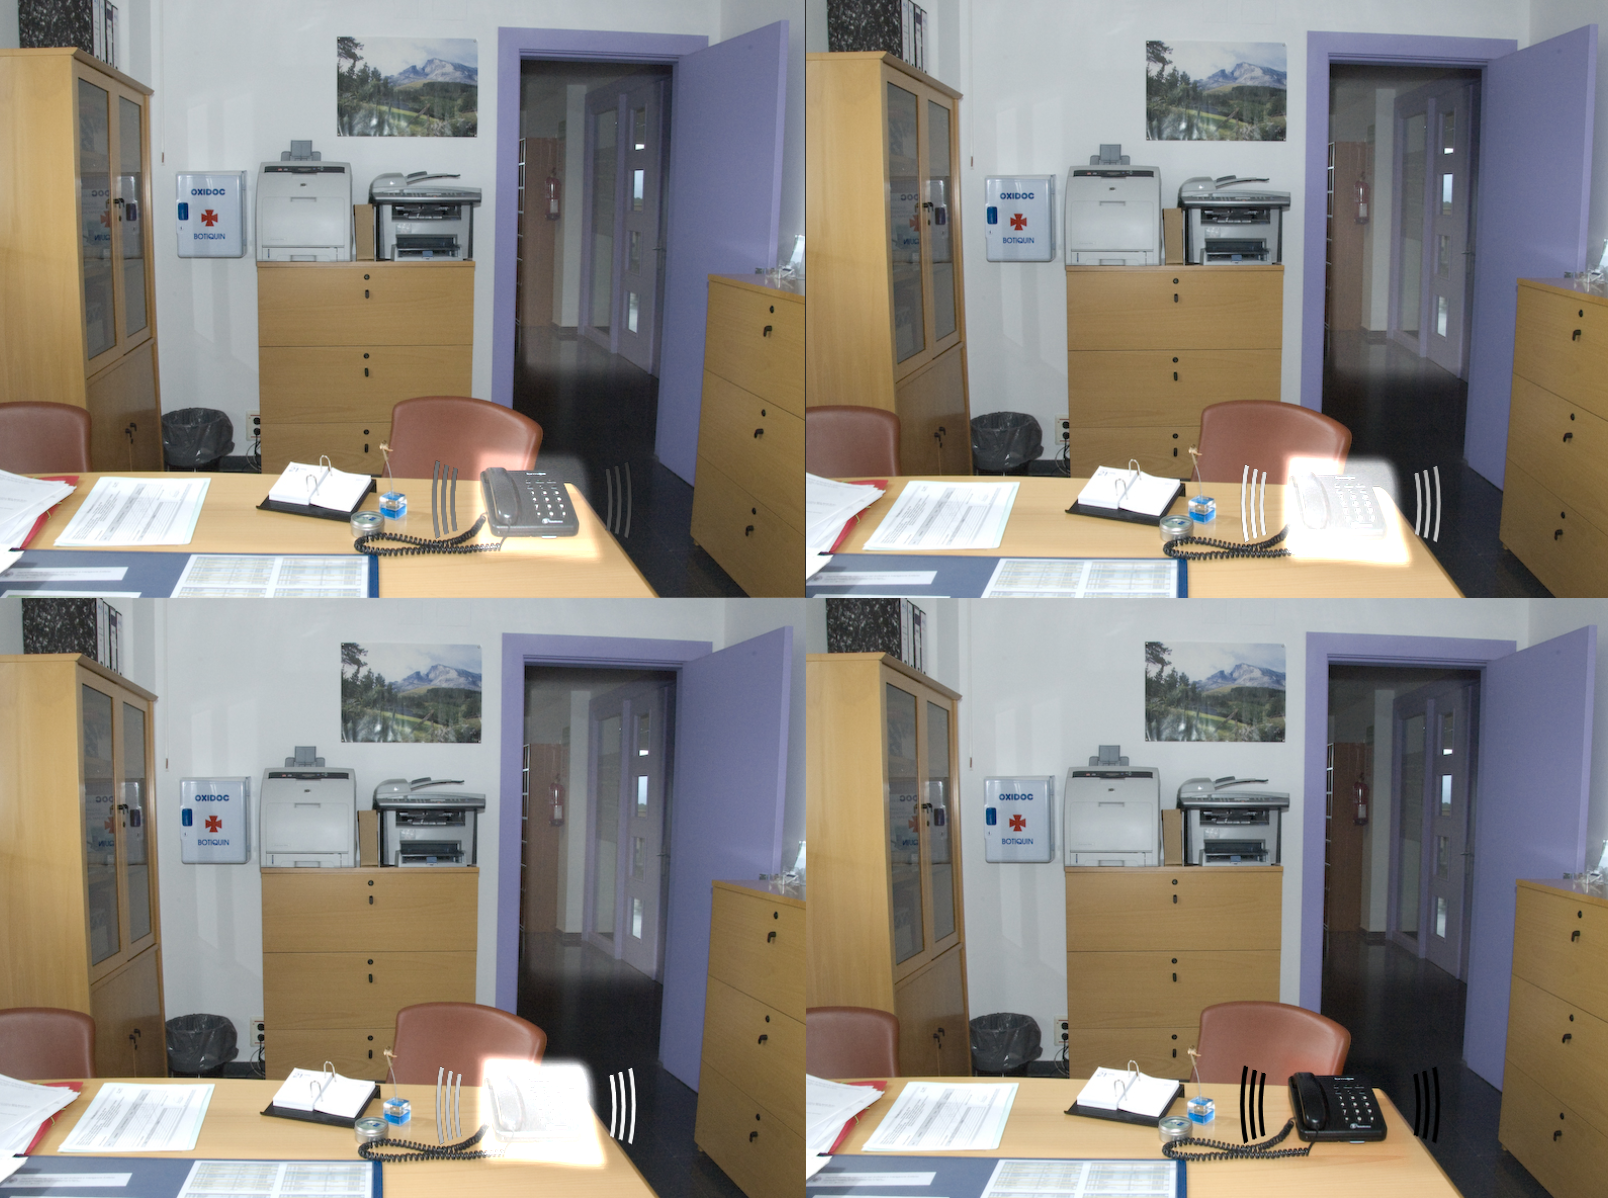
\includegraphics[width=4.3in]{figures/it2/apearance/fire.png}}
	\caption[Apearance - Versión Final]{Diagrama de clases de Apearance, sin incluir Bubble.}
	\label{autoglow2it2}
\end{figure}

\begin{figure}[h!]
	\centerline{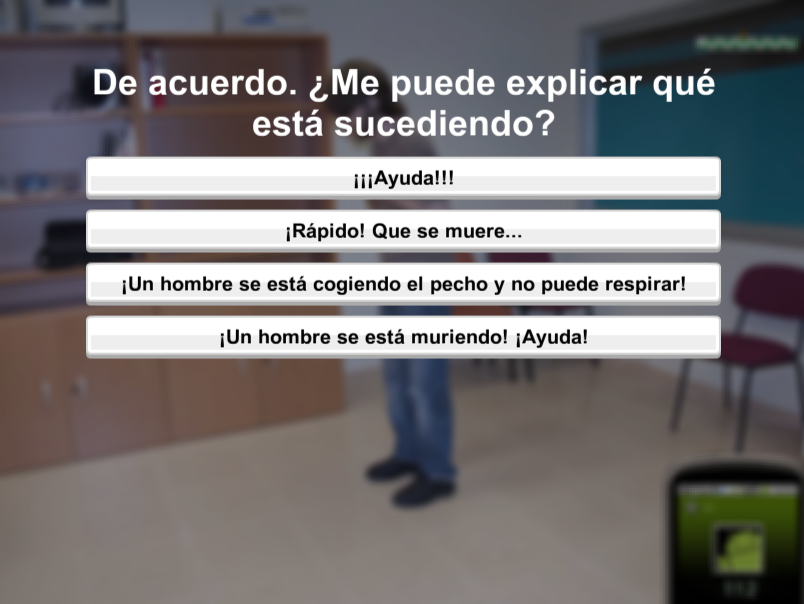
\includegraphics[width=4.3in]{figures/it2/apearance/blur.png}}
	\caption[Apearance - Versión Final]{Diagrama de clases de Apearance, sin incluir Bubble.}
	\label{blurit2}
\end{figure}

\subsubsection{El menú contextual de acciones: Menu}

El menú contextual es uno de los elementos que existían antes y que ha sido recreado, añadiendo animación al mismo para que su representación visual sea más sencilla. La utilidad del menú contextual es mostrar acciones en forma de botones para que el usuario pueda pulsarlos y ejecutar las acciones que están detrás de los mismos.

Este menú contextual se genera utilizando una de las funciones de \textit{GUIManager}, la función \textit{showActions(list<Action>)} que, inicializa el menú y utiliza su función \textit{regenerate()}, que lo que hace es, en función de los parámetros que se le hayan establecido, genera nuevos botones, y los coloca para que se animen correctamente. Tras esto la clase \textit{OptionMB} se encarga de ir colocando tanto la línea que une el centro del menú con el botón, como el botón en si mismo. Asimismo, esta clase establece la acción en \textit{ButtonMB}, clase que implementa la interfaz \textit{Interactuable}, y que permite al usuario interactuar con ella. Es la clase \textit{ButtonMB} la que se encarga de modificar su representación en función de la imagen que le provea el \textit{GUIManager}. Esto está representado en la figura \ref{menuit2}, donde participan \textit{MonoBehaviour} e \textit{Interactuable}.

\begin{figure}[h!]
	\centerline{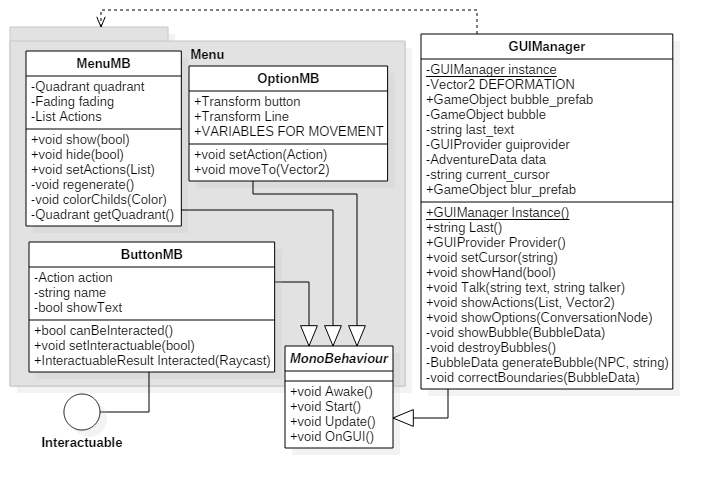
\includegraphics[height=3.3in]{figures/it2/Menu.png}}
	\caption[Menu - Versión Final]{Diagrama de clases de Menu, incluyendo las relaciones que tienen con MonoBehaviour e Interactuable.}
	\label{menuit2}
\end{figure}

Finalmente, en la figura \ref{menuvisualit2} muestra el menú generado en una situación en la que se pueden realizar cinco acciones sobre un elemento de la escena. 

\begin{figure}[h!]
	\centerline{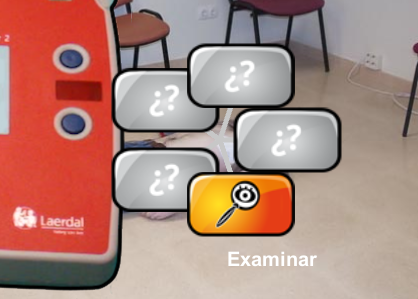
\includegraphics[height=3in]{figures/it2/apearance/menu.png}}
	\caption[Visual Menu - Versión Final]{Imagen de la representación visual del menú.}
	\label{menuvisualit2}
\end{figure}

\subsection{El gestor de recursos: ResourceManager}
\label{resourcemanager}

Como se ha comentado varias veces a lo largo de esta sección, para facilitar el acceso a los recursos desde cualquier parte del proyecto, existe un \textit{Singleton} llamado \textit{ResourceManager} que provee de elementos multimedia al que lo solicite.

Este \textit{ResourceManager} es capaz de cargar múltiples tipos de recursos, y para ello utiliza métodos diferentes. Asimismo, existen dos formas de cargar recursos, y las clases que se encargan de acceder al sistema de archivos para cargar los recursos se adaptan a estos tipos.

Estos tipos de carga, o \textit{LoadingType}, son: utilizando el sistema de ficheros del sistema operativo, mediante la librería \textit{System.IO}, teniendo la ventaja de que, una versión ya generada de uAdventure puede cargar cualquier juego que se establezca en un directorio determinado; y por otra parte, utilizando \textit{Resources.Load()}, mediante el sistema de ficheros de Unity, que tiene la ventaja de que estos archivos, una vez que se produce una \textit{Release} del proyecto, están incluidos en un paquete comprimido por Unity, y permiten instalar uAdventure junto al juego en cualquier plataforma sin tener que preocuparse de incluir el juego.

\begin{figure}[h!]
	\centerline{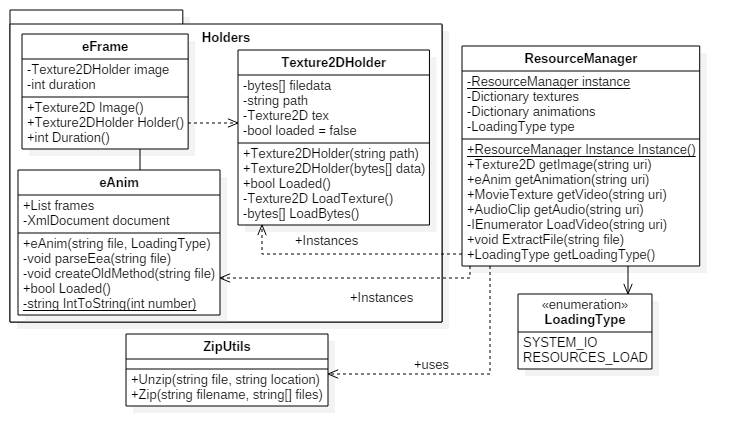
\includegraphics[height=3.5in]{figures/it2/ResourceManager.png}}
	\caption[ResourceManager - Versión Final]{Diagrama de clases de ResourceManager junto a los cargadores de recursos.}
	\label{resourcemanagerit2}
\end{figure}

con respecto a los tipos de ficheros que se pueden cargar con \textit{ResourceManager},encontramos los siguientes tipos:
\begin{itemize}
	\item \textit{Imágenes}: Para la carga de imágenes existe una clase llamada \textit{Texture2DHolder}. Dependiendo del tipo de carga que utilice \textit{ResourceManager}, o bien se carga la textura directamente con \textit{Resources.Load()}, o bien se leen los \textit{bytes} de dicho fichero, para más adelante transformarlos en una \textit{Texture2D}.
	
	\item \textit{Animaciones}: Las animaciones que se cargan son las de eAdventure, y están compuestas por una serie de imágenes, esto se hace en la clase \textit{eAnim}, la cual no ha cambiado mucho en su funcionamiento desde lo explicado en la sección \ref{dataclassesit1}. Para añadir soporte a \textit{Resources.Load()} ha sido necesario implementar un método que renombra todos los archivos ".eaa" a ".xml" pues Unity no reconoce dichos archivos como ficheros de texto y no permite cargarlos.
	
	\item \textit{Vídeos}: La carga de vídeos se realiza almacenándolos en una \textit{MovieTexture}. Para la carga de estos desde el sistema de ficheros se utiliza la clase \textit{www}, que permite hacer solicitudes POST y GET, ya sea en local, al sistema de ficheros, o a un servidor. Esta carga requiere la utilización de corrutinas, pues sin ellas el juego se quedaría completamente congelado hasta que el recurso estuviera cargado. Finalmente mencionar que los vídeos únicamente pueden estar en formato ".ogv" bajo el codec OGG Theora.
	
	\item \textit{Audio}: De manera similar a los vídeos, se utiliza la clase \textit{www} para su carga, aunque en esta ocasión son almacenados en \textit{AudioClip}.
	
	\item \textit{Archivos Zip}: Estos ficheros técnicamente no son cargados en tiempo de ejecución, sino que son extraídos bajo demanda del emulador para importar juegos. Estos juegos deben estar en formato ".jar", y únicamente se extrae de ellos la parte necesaria. Más detalles acerca de este proceso están disponibles en la sección \ref{emulatorit3}.
\end{itemize}

Acerca de los vídeos, y de la importación de los juegos que se realiza en la tercera iteración del proyecto, se realizó una investigación acerca de la posibilidad de transformar dichos vídeos en el proceso de importación del juego. Los resultados no fueron satisfactorios, pero abrieron varias puertas para abordar este problema.

En primer lugar, se probaron multitud de librerías que facilitaban la conversión de vídeos a sistemas .NET, sin embargo, ya que Unity utiliza una versión reducida del mismo, dichas librerías fallaban en tiempo de ejecución y no completaban la conversión del vídeo. Por otra parte, algunas personas que se han enfrentado al mismo problema, han generado \textit{Wrappers} que utilizan un ejecutable del proyecto de software libre \textit{FFMPEG}, que provee de una serie de utilidades para transformar vídeos fácilmente.

Se intentaron incorporar dichos \textit{Wrappers} en el proyecto, pero ninguno de ellos funcionó. Finalmente se decidió que la alternativa de implementar un \textit{Wrapper} muy sencillo, con únicamente la funcionalidad de transformar a OGV, sería la opción mas viable. en windows, esto se haría de la siguiente manera:

\begin{lstlisting}
String path = @"f:\temp\data.txt";
Process foo = new Process();
foo.StartInfo.FileName = "Notepad.exe";
foo.StartInfo.Arguments = path;
foo.Start();
\end{lstlisting}

También existe una manera de lanzar clases Java directamente desde Unity, pudiendo realizar este proceso también en Android, de la siguiente manera:

\begin{lstlisting}
using (AndroidJavaClass ext = new AndroidJavaClass ("com.external.class")) 
{
	ext.CallStatic ("whatever", Parameter1, Parameter2);
}
\end{lstlisting}

Por lo que, como trabajo futuro del proyecto, queda pendiente implementar dicho conversor de vídeos multiplataforma, que utilice diferentes librerías, ya sea \textit{FFMPEG} u otra librería para dicha conversión.

\section{El modelo de Datos: Core}
\label{coreit2}

En el proceso de integración del proyecto de Piotr Marszal que consiste en reconstruir el editor de eAdventure dentro de Unity, se decidió unificar el modelo de datos. En vista de que, para una implementación al completo de todos los elementos del editor, el modelo de datos planteado en la sección \ref{dataclassesit1}, con las clases de datos que eran capaz de generarse a si mismas, era insuficiente para satisfacer las necesidades del proyecto, se decidió invertir mucho tiempo en portar al completo el modelo de datos de las clases Java a Unity.

Esta tediosa y repetitiva labor fue realizada casi en su totalidad por Piotr, quien copiaba el código Java en c\# y se encargaba de sustituir las librerías problemáticas por librerías análogas de .NET. Dentro de mi aportación, se realizaron tareas de corrección de errores y de pruebas para comprobar que todo funcionaba correctamente.

De esta misma manera, Piotr importó el \textit{Loader} original de eAdventure, y, no fue hasta que se comenzó a utilizar en este proyecto, que no se identificó que dicho cargador era inviable de utilizar pues tardaba entre medio y un minuto en leer el documento de especificación del juego; además de que lo hacía con errores que, pese a intentos de arreglarlos, debido a que la implementación de dicho \textit{Loader} fue realizada por uno de los desarrolladores de eAdventure, la complejidad del funcionamiento del mismo se escapaba a nuestra comprensión.

Como estos problemas con el \textit{Loader} continuaban, se decidió crear una nueva implementación del cargador del modelo de datos utilizando la librería \textit{System.XML} que se utilizó para las Clases de datos de la primera iteración, y que ya se conocía que era fácil de utilizar, pues permite utilizar sintaxis de XPath\footnote{XPath (XML Path Language) es un lenguaje declarativo que permite construir expresiones regulares que recorren, procesan y seleccionan elementos de un documento XML}, y acceder al contenido del documento XML de forma sencilla.

Esta segunda implementación la comenzó Piotr, recodificando la mayor parte de \textit{subparsers} del cargador. Sin embargo, el no pudo probar las nuevas clases que estaba implementando, por lo que no pudo darse cuenta de que muchas de ellas, debido a que la base que aplicaba para la transformación no era del todo correcta, no funcionaban. Los grandes \textit{subparsers} como el cargador de escenas, efectos, conversaciones, areas activas, etc... tuvieron que ser nuevamente implementados desde cero por mi. Finalmente, en mi labor se realizó la tarea de implementar los cargadores principales de \textit{AdventureData} y \textit{Chapter}. haciendo estos funcionales al sistema de cargado de ficheros de \textit{System.IO}, así como el de \textit{Resources.Load()}.

Una vez construido el nuevo \textit{Loader}, los tiempos fueron reducidos en un 90\%, pasando de tardar 45 segundos de tiempo de carga en el videojuego \textit{Checklist}, a alrededor de 4 segundos. No obstante esta medida no puede realizarse con precisión debido a que en dichos tiempos de carga se incluye el tiempo que utiliza Unity para inicializarse y ponerse en funcionamiento.

Para completar la integración fue necesario desacoplar partes del sistema de eAdventure entre si mismas, pues el modelo de datos de dicho sistema está extremadamente interconectado, y cada vez que se intenta reutilizar una de sus partes, es necesario traer junto a esa parte, un gran número de partes de dicho modelo. 

Con dicho desacoplamiento, también fueron eliminados del modelo de datos determinados elementos utilizados para iniciar la carga del juego. Por ello fue necesaria una investigación en profundidad hasta hallar una manera segura de trabajar con el paquete \textit{Loader}.

Finalmente, cuando se hubo unificado el modelo de datos, se realizó una unión de ambos proyectos en un único proyecto y repositorio. El proyecto de Piotr se ubica casi en su totalidad dentro del espacio de nombres \textit{Editor}, por lo que, para la unificación de los proyectos, fue necesario extraer de dicho espacio de nombres el modelo de datos, junto al \textit{Loader}, otras clases auxiliares, y más elementos. A esta parte que se extrajo de \textit{Editor} es a la que se conoce como \textit{Core}, pues representa al núcleo de eAdventure.

\newpage

\section{La comunicación con RAGE: RAGETracker}
\label{ragetrackerit2}

Pese a que uno de los objetivos principales de este proyecto es el de garantizar y simplificar el ciclo de vida de los juegos serios producidos con eAdventure, así como extender su vida útil lo máximo posible, otro de los planteamientos con los que surge este proyecto es el de poder mejorar la parte de evaluación de eAdventure mediante el uso de RAGE.

Una de las partes que, por tener un grado de dificultad muy elevado de incluir en Unity, debido a que las librerías que se utilizaban no dan soporte a .NET, y se debe construir una nueva infraestructura para soportarlo, es la parte de \textit{Assessment}. Estas partes, que además no tenían toda la funcionalidad deseada, van a ser sustituidas por \textit{Assessment} con RAGE.

RAGE, Realising an Applied Gaming Eco-system, es un proyecto que apunta a desarrollar, transformar y enriquecer tecnologías específicas para la industria de los videojuegos serios, en forma de paquetes autocontenidos para juegos que ayudan a los estudios de videojuegos en el desarrollo de juegos serios, haciéndolo más sencillo, rápido y eficiente económicamente.

En RAGE hay una parte específica dedicada a la evaluación de videojuegos, y esta parte provee una API para los profesores que deseen crear perfiles de evaluación y progreso, así como otros elementos de utilidad que se deseen monitorizar, como el numero de veces que una pregunta ha sido respondida de forma incorrecta, o los días que los estudiantes han sido más activos jugando a un videojuego.

En eAdventure, este proceso de evaluación se realiza mediante la especificación de una serie de frases de evaluación, en lenguaje natural, que, cuando se den una serie de condiciones, serán incluidas en un registro de evaluación. Este registro se muestra al jugador al terminar el juego, y este debe enviar dicho registro al profesor, o debe ser revisado por el profesor al terminar la clase.

Este proceso tiene multitud de problemas, entre los cuales podemos encontrar: casos como que, el profesor nunca llegue a ver dicho registro de evaluación, ya sea porque el alumno decida no enviar dicho registro al profesor, o porque el alumno lo cierre sin querer; problemas a la hora de evaluar porque no sea suficientemente específico en el desarrollo del juego; o el gran problema de que, para poder realizar la evaluación, es el propio desarrollador el que tiene que incluir elementos de evaluación dentro del juego. Sin embargo, todos estos problemas son asumibles, porque se entiende que el profesor va a tener tiempo para dedicar a cada alumno, hablar con él en caso de que tenga dudas acerca del desarrollo del juego, y que los juegos desarrollados, en general, son de corta duración, y pueden ser completados de inicio a fin en una sesión.

Pero, ¿Qué ocurre si pasamos de tener el ámbito de una clase, a una cantidad de alumnos que sobrepasa el límite del profesor? ¿Podría leer los registros de todos los alumnos y evaluar uno por uno? La respuesta es no, o al menos no de forma apropiada. Por ello, es necesario que este proceso de evaluación sea rediseñado y reconstruido utilizando las ventajas que RAGE provee a los desarrolladores de juegos. Delegando este proceso de evaluación, y únicamente monitorizando las desviaciones que sufren los alumnos, se podrá conseguir que el proceso de evaluación de un número de alumnos elevado, mediante el uso de un juego generado por uAdventure, se realice de forma sencilla y cómoda.

Además de las ventajas que RAGE proveerá a uAdventure, el segundo se encargará de facilitar la generación de estos perfiles de evaluación desde el propio editor de uAdventure. Un ejemplo de este proceso automatizado sería, la generación del progreso del usuario dentro del juego a través del árbol de escenas que comunica la escena inicial con la escena final. También se podrían marcar variables importantes para el desarrollo del juego, para su monitorización, y se generarían gráficas de su evolución, así como poder generar alertas si una de dichas variables se saliese de un rango apropiado. Finalmente, se intentaría preservar el antiguo sistema de alertas de eAdventure, utilizando el sistema de alertas de RAGE.

Recalcar también que, RAGE no únicamente permite facilitar la evaluación al profesorado, sino que también ayuda a investigadores y desarrolladores, permitiendo generar estadísticas como las preguntas más falladas, y la opción más elegida dentro de ellas; generación de mapas de calor dentro de una escena, para saber las zonas donde más interactúa el usuario, o saber las escenas donde el jugador pierde más el tiempo, o le resultan más complejas de superar.

En cuanto a la funcionalidad que \textit{RAGETracker} aporta en si mismo, únicamente facilita el proceso de comunicación con RAGE. Implementa unas clases que realizan la conexión con el API, autorizan al usuario mediante un \textit{Token} de identificación, y relacionan el juego al que se está jugando, con un juego dado de alta en RAGE. La implementación de dicho \textit{Tracker} está disponible en \url{https://github.com/e-ucm/unity-tracker}.
%\chapter{Tercera Iteración: El Emulador y los editores}

Como se explica en el la subsección \ref{metodologiadedesarrollo}, en la que se expone la metodología de desarrollo utilizada para el proyecto, este sufre de tres grandes iteraciones para su completitud. En esta sección se explican los detalles implementados en la tercera iteración, es decir, la generación de un emulador de juegos e eAdventure, utilizando el núcleo de ejecución \textit{Runner} explicado en la sección \ref{runnerit2}, y el modelo de datos de eAdventure explicado en \ref{coreit2}; además de la generación de editores para el editor de uAdventure desarrollado por Piotr Marszal. 

\section{El Emulador de Juegos}
\label{emulatorit3}

Uno de los principales problemas de todo software consiste en que, el presupuesto que se invierte en el desarrollo de dicho software, no debe invertirse por completo en su desarrollo, pues la vida útil del mismo durará varios años más, en los que debe haber un mantenimiento y soporte para dicho software. El software producido por eAdventure, en muchos casos, hace años que dejó de tener soporte, pues no sólo los desarrolladores abandonaron los proyectos, sino que eAdventure no sufre ninguna actualización desde el 29 de Octubre de 2012, y todos los errores que han surgido, y los problemas de soporte que tiene en diferentes dispositivos han limitado la vida útil del software producido con eAdventure, y su ciclo de vida.

uAdventure, construido sobre Unity3D permite abrir proyectos de eAdventure, y videojuegos ya generados, dando la posibilidad de modificarlos, y probarlos sobre el nuevo núcleo de ejecución, ampliando y simplificando el ciclo de vida del videojuego. Tras haber abierto dicho juego, mediante las herramientas de compilación de Unity3D, se puede generar un paquete standalone con el juego en su interior.

No obstante, muchos proyectos han sido completamente abandonados, y es posible que nadie decida transformar un juego, o que, por desconocimiento de su existencia, no se transforme a uAdventure. Por todo ello, este framework puede ser compilado en sí mismo como un emulador de juegos de eAdventure, permitiendo al usuario explorar su sistema de ficheros, e importar de forma sencilla aquellos juegos que desee jugar.

Este emulador evoluciona de una prueba incluida en la clase controladora del juego en el prototipo generado en la primera iteración. Esto consistía en permitir al usuario seleccionar un juego de una lista de juegos disponibles en lugar de lanzar directamente un juego especificado en la clase controladora. En este primer prototipo la interfaz era muy sencilla, sin opciones, y no permitía técnicamente importar juegos, sino que debían de importarse descomprimiendo los juegos en una carpeta determinada del sistema de ficheros. Además, incluía un diálogo de carga que mostraba el progreso de la carga del juego.

Esta primera versión del emulador se muestra en la figura \ref{betaemuit3}.

\begin{figure}[htb]
	\centerline{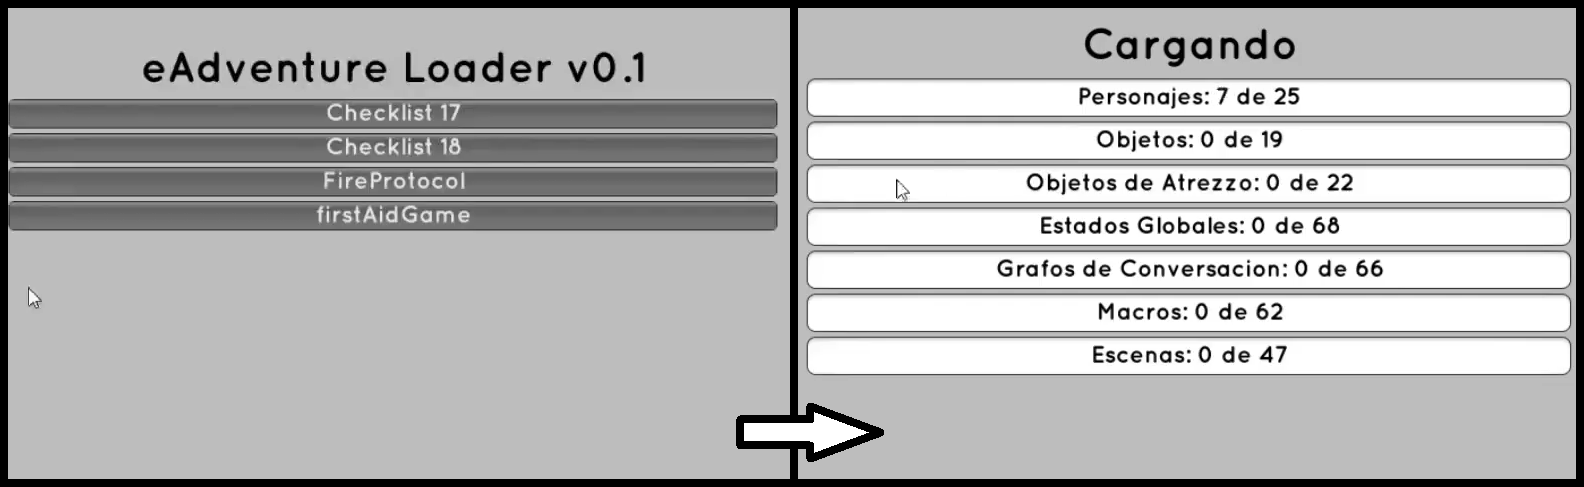
\includegraphics[height=2in]{figures/it3/betaemu.png}}
	\caption[Primer prototipo - Emulador]{La parte de la izquierda muestra el menú principal del primer prototipo del emulador. Una vez seleccionado un juego, se mostraba un diálogo de carga como el que se ve en la parte derecha.}
	\label{betaemuit3}
\end{figure}

No obstante, y dado que esta primera versión del emulador era insuficiente, además de que el diálogo de carga de ficheros no permitía ser ejecutado si se utiliza el sistema de carga de recursos de Unity3D, \textit{Resources.Load()}, este emulador evolucionó en 5 vistas:

\begin{itemize}
	\item \textbf{Menú Principal}: El menú es la puerta de entrada al emulador. Cuando se pone en funcionamiento muestra en el centro un catálogo de juegos instalados, si los hay. Pulsando sobre cualquiera de estos juegos comienza la ejecución del mismo. Finalmente, en la parte inferior de la vista hay 3 botones que permiten acceder a más vistas del emulador. Cada juego presentado en el menú principal tiene un icono que lo representa. La obtención de dicho icono se hace explorando los archivos incluidos dentro del directorio \textit{/gui/} en busca de un fichero llamado "standalone\_game\_icon.png", si dicho fichero no existe, se selecciona el icono de la versión de eAdventure con la que fue generado dicho juego, incluido también en el mismo directorio.

\begin{figure}[h!]
	\centerline{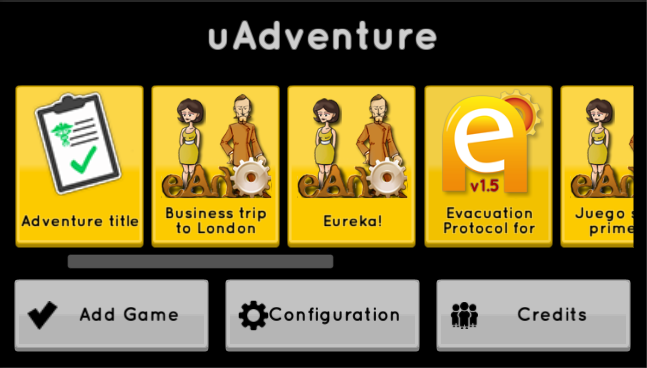
\includegraphics[height=2.5in]{figures/it3/emu-main.png}}
	\caption[Menu Principal - Emulador]{Vista del menú principal del emulador de uAdvneture.}
	\label{emumainit3}
\end{figure}


	\item \textbf{Explorador de Archivos}: Dado que Unity no provee, en tiempo de ejecución, de una manera de seleccionar un fichero del sistema de archivos, se ha implementado desde cero un explorador de archivos. Este permite navegar por carpetas, las cuales se ven en un color amarillo, y seleccionar juegos para ser añadidos. Estos juegos se representan con el icono de un mando de videojuegos, y con un color azul. Tras seleccionar un juego se puede pulsar el botón \textit{Add Game}, que lanza la vista que se presenta a continuación.

\begin{figure}[h!]
	\centerline{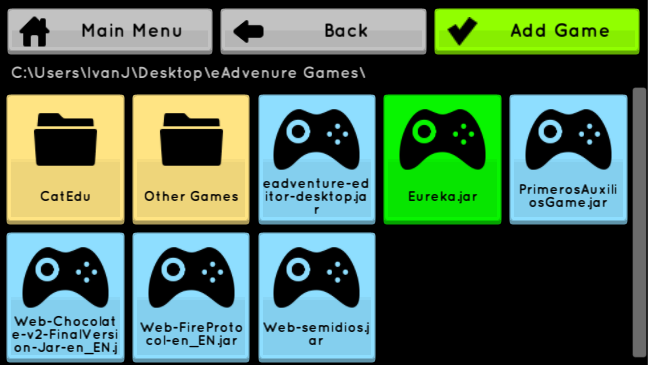
\includegraphics[height=2.3in]{figures/it3/emu-file.png}}
	\caption[Explorador de Archivos - Emulador]{Vista del explorador de archivos del emulador de uAdventure.}
	\label{emufileit3}
\end{figure}

	\item \textit{Importador de juegos}: Pese a que esta sea una de las vistas más sencillas, pues únicamente muestra un texto y una pequeña animación de tres puntos moviéndose, tras esta animación se encuentra el proceso de importado del juego. En el que se descomprimen las partes necesarias, y se borran algunos elementos tras su descompresión. Como se explicó en la sección \ref{resourcemanagerit2}, la transformación de los vídeos se realizaría en esta escena.
	
\begin{figure}[h!]
	\centerline{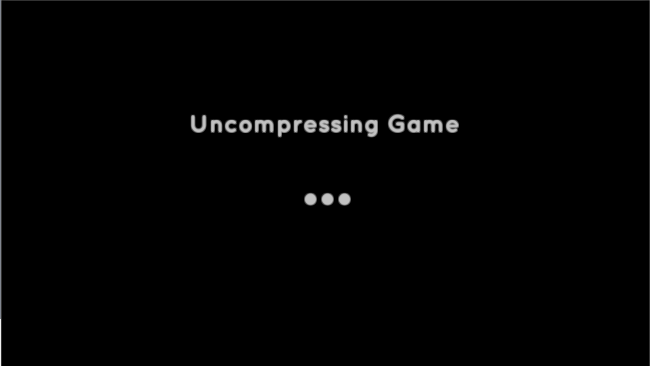
\includegraphics[height=2.3in]{figures/it3/emu-loader.png}}
	\caption[Importador de Juegos - Emulador]{Vista del importador de juegos del emulador de uAdventure.}
	\label{emuloaderit3}
\end{figure}
	
	\item \textit{Configuración}: La ventana de configuración provee al usuario de la capacidad de poder modificar el funcionamiento del intérprete, pudiendo configurar tres apartados: Gráficos, Sonido y Otros. Dentro del apartado gráfico se permite la posibilidad de deshabilitar los \textit{Shaders} explicados en la sección \ref{apearanceseccionit2}, así como deshabilitar los vídeos, o las animaciones. Dentro del apartado de sonido se permite configurar el uso de audio, así como su volumen y si se desea, forzar el uso de \textit{Text To Speech}, texto hablado. Finalmente, en el apartado de otras configuraciones, se permite modificar la velocidad del texto en las burbujas, así como la posibilidad de dehabilitar RAGE, o la persistencia de ficheros multimedia, para reducir el uso de memoria de la aplicación.
	
\begin{figure}[h!]
	\centerline{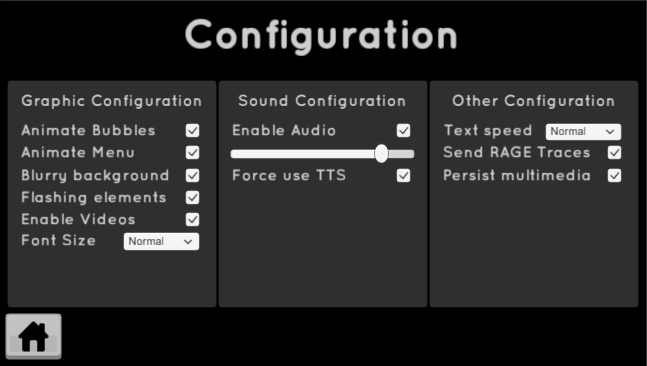
\includegraphics[height=2.3in]{figures/it3/emu-config.png}}
	\caption[Configuración - Emulador]{Vista de configuración del emulador de uAdventure.}
	\label{emuconfigit3}
\end{figure}
	
	\item \textit{Créditos}: La vista de créditos contiene el listado de las personas que han participado, dirigido o realizado aportaciones tanto a uAdventure como a eAdventure.
	
\begin{figure}[h!]
	\centerline{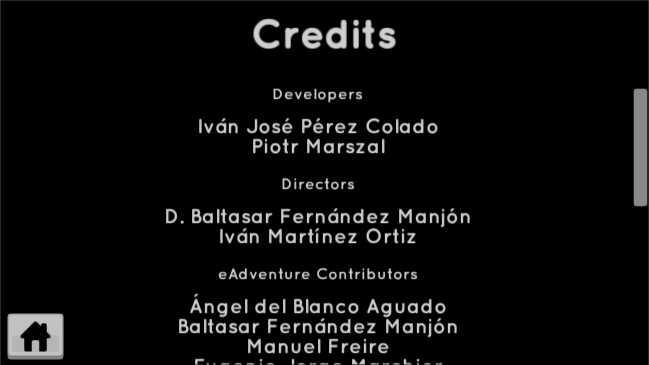
\includegraphics[height=2.3in]{figures/it3/emu-credits.png}}
	\caption[Créditos - Emulador]{Vista de los créditos presentados en el emulador de uAdventure.}
	\label{emucreditsit3}
\end{figure}

\end{itemize}

\section{Los Editores de Secuencias}

Como parte del proceso de integración de los proyectos, y para realizar un aporte comparable al esfuerzo que Piotr había realizado al importar el modelo de datos de eAdventure, en el desarrollo de este proyecto se generaron dos editores basados en ventanas para la edición de las secuencias.

Dada la experiencia de generación de editores de este estilo obtenida durante el desarrollo del TFG IsoUnity, que consistía en la generar un editor de videoaventuras en tercera persona con estilo isométrico, en el que se incluyen editores que presentan similitudes con dichas necesidades, el desarrollo de dichos editores será más sencillo.

Las clases de eAdventure que requieren editores son: Los efectos, que pese a ser lineales, se plantea la posibilidad de incluir bifurcaciones que los transformen en un grafo en un futuro; Las conversaciones, que son grafos de diálogo con nodos de conversación que incluyen diálogo o opciones de respuesta; y el editor de condiciones, que al ser tan pequeño se explicará como parte del editor de efectos.

Para el desarrollo de cada uno de estos editores se implementarán tres clases cruciales:

\begin{itemize}
	\item La ventana principal del editor, que es capaz de gestionar la secuencia en si misma, compuesta por un listado de nodos, y de mantener en orden las ventanas que representan los editores individuales de cada uno de los nodos.
	
	\item Una interfaz que permita implementar editores para los nodos, con métodos para pintarse utilizando la GUI de editor de Unity, y métodos que permiten identificar si un editor sirve para representar un tipo de nodo, y clonarse a si mismo.
	
	\item Finalmente, una factoría que explore el espacio de nombres utilizando Linq, en busca de editores que implementen la interfaz para generar editores de nodo. Dicha factoría también tiene que proveer un listado de los editores disponibles, así de facilidades para instanciar un editor para un nodo concreto. Existen detalles acerca de la implementación de factorías utilizando esta técnica en la sección \ref{linqit1}
\end{itemize}

Con estas tres clases, ya se pueden generar editores individuales para los nodos, consiguiendo un editor de secuencias muy extensible, preparado para añadir nuevos editores de forma sencilla y sin necesidad de modificar ninguna de las clases. Generando una nueva clase que implemente la interfaz del editor, este ya la identificaría y añadiría a su listado de editores disponibles.

\subsection{El Editor de Efectos}

Entre los editores de secuencias implementados, el más sencillo, pero a su vez más largo de implementar es el editor de efectos, pues estos son una secuencia lineal, no son ni árboles, ni grafos, por lo que la implementación de un editor con ventanas lineal se plantea sencilla. Sin embargo, la cantidad de editores de efectos que se deben implementar es muy elevada, pues existen multitud de efectos que implementan la interfaz \textit{AbstractEffect}.

Para la implementación de esta ventana de editor, se extiende la clase abstracta \textit{EditorWindow} que provee una serie de métodos que, de implementarse, permiten la generación de una nueva ventana para el editor. En primer lugar, una funcion Init() que inicializa la ventana para un efecto dado. Una funcion \textit{nodeWindow(int id)} que se encarga de gestionar cada ventana individualmente. Unas funciones \textit{CreateWindows()} y \textit{CreateWindow(AbstracEffect effect)}, que son las encargadas de generar las ventanas para los efectos. Una funcion \textit{curveFromTo()} que genera una línea entre dos ventanas, y finalmente, la función \textit{OnGUI()} que ejecuta todo lo anterior para generar la ventana.

En la figura \ref{mainwindow-effecteditor-it3} se ve una secuencia de efectos sencilla, compuesta por 5 efectos en los que se establece valor para unas variables, el jugador habla, y finalmente, se lanza una conversación completa. El menú desplegable muestra todos los editores de efectos implementados. En la parte de arriba de la figura se observa un botón muy ancho con el texto "New Effect", que sirve para añadir un nuevo nodo a la lista de efectos. En esta ventana, las subventanas que permiten la edición de efectos se pueden mover, por lo que permiten la organización de los mismos de la forma más conveniente.

\begin{figure}[h!]
	\centerline{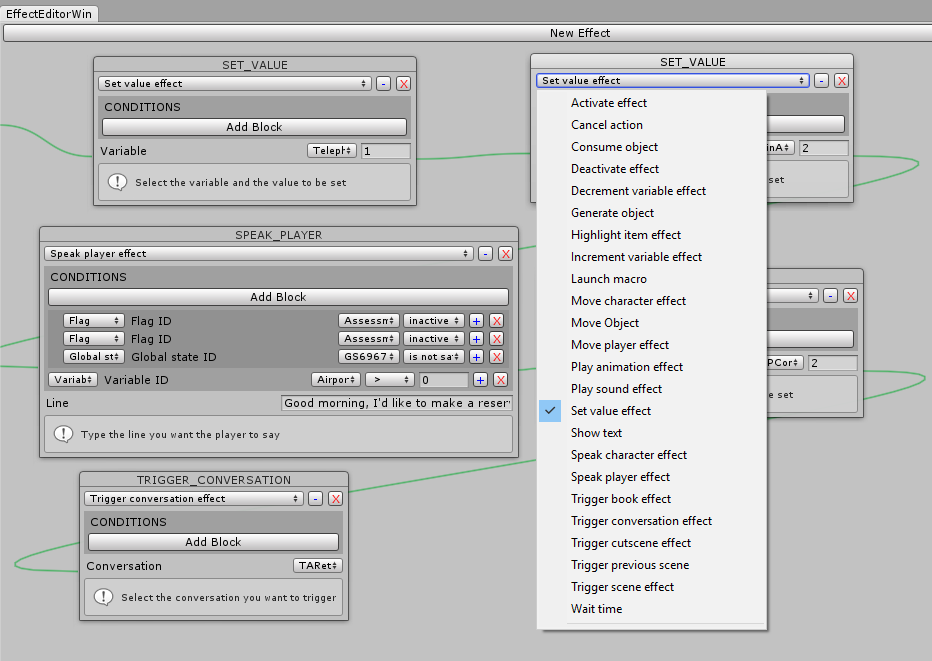
\includegraphics[height=4in]{figures/it3/effecteditorwindow.png}}
	\caption[Ventana Principal - Editor de Efectos]{Ventana principal del editor de efectos.}
	\label{mainwindow-effecteditor-it3}
\end{figure}

En la figura \ref{effect-nodes-it3} se muestra un nodo de efecto que muestra una gran cantidad de condiciones para su ejecución. Este nodo puede reducirse en tamaño para facilitar la edición mediante el botón con el guión de color azul, transformándose en la ventana derecha.

\begin{figure}[h!]
	\centerline{
		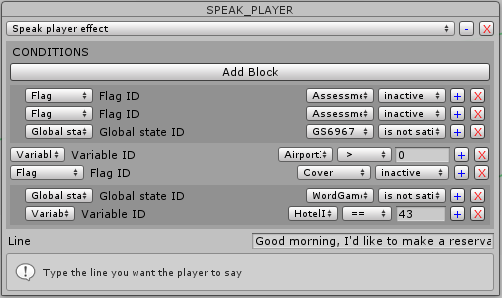
\includegraphics[height=2.5in]{figures/it3/editor-conditions.png}
		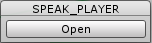
\includegraphics{figures/it3/collapsed-effect.png}
		}
	\caption[Editor de Nodo con condiciones - Editor de Efectos]{Editor de nodo de efecto con condiciones, vista normal y reducida.}
	\label{effect-nodes-it3}
\end{figure}

\subsection{El Editor de Conversaciones}

Pese a que en primera instancia parece que el editor de conversaciones es muy similar al editor de efectos, y aunque visualmente lo sean, las conversaciones son grafos, y la modificación de un editor que trabaja con listas, a un editor capaz de trabajar con grafos direccionales, no es una tarea trivial. 

Las modificaciones, con respecto al editor de efectos están relacionadas con la gestión de ciclos en los grafos, y la posibilidad de generar hijos para nodos concretos, así como permitir al usuario establecer el hijo de un nodo directamente, mostrando en la interfaz cual es la rama de nodos que, si no tiene ningún otro nodo padre, se va a perder, y cual es la nueva rama que se va a establecer como hija de dicho nodo.

Como en el desarrollo de este editor no era tan necesario generar un gran número de editores, pues las conversaciones únicamente están compuestas por editores de diálogos y de opciones, dichos editores cuentan con un acabado mucho más conseguido, reutilizando muchas de las imágenes de la interfaz de eAdventure. Esto se muestra en la figura \ref{small-dialogeditor-it3}, en la que, además, se muestra lo descrito en el párrafo anterior. La línea azul será el nuevo hijo, y la roja el hijo descartado.

\begin{figure}[h!]
	\centerline{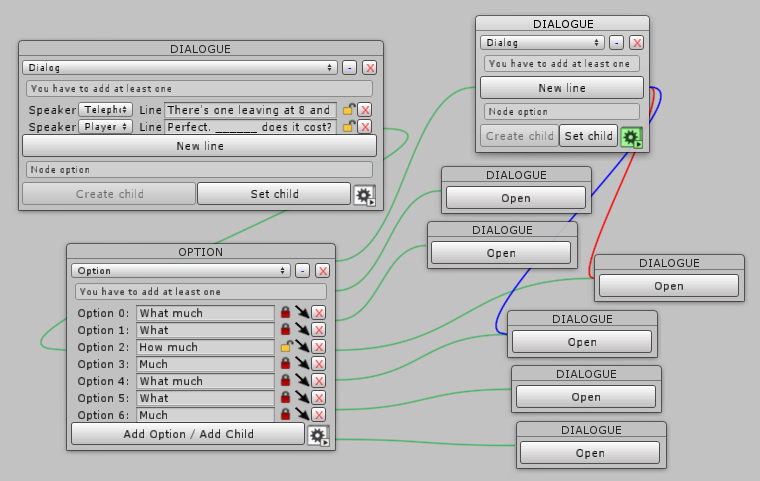
\includegraphics[height=3in]{figures/it3/small-dialog.png}}
	\caption[Pequeño diálogo - Editor de Diálogos]{Pequeño diálogo mostrado en el editor de diálogos.}
	\label{small-dialogeditor-it3}
\end{figure}

Como detalle adicional, se ha generado una clase llamada \textit{NodePosicioner} que, estableciendo un número de nodos, y una altura de la ventana, posiciona automáticamente los nodos en su lugar correspondiente automáticamente, de manera que ver las secuencias es más cómodo si se abren y no existen datos acerca de su posición. Esto se muestra en la figura \ref{circle-nodes-it3}.

\begin{figure}[h!]
	\centerline{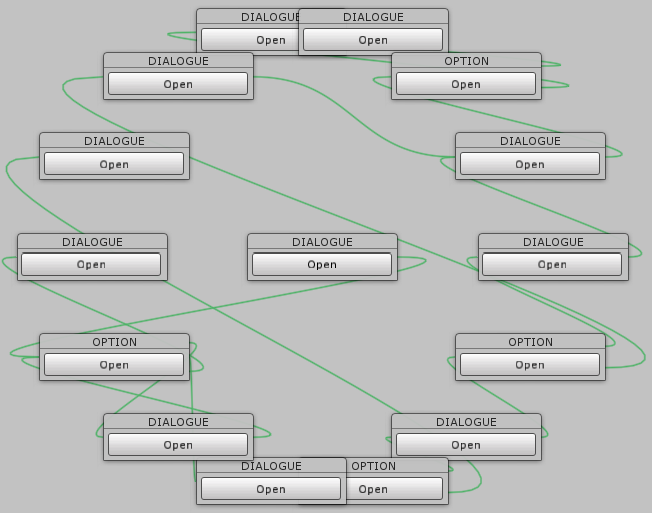
\includegraphics[height=2in]{figures/it3/nodes-circle.png}}
	\caption[Anillo de nodos - Editor de Diálogos]{Posicionamiento automático de nodos en el editor de diálogos.}
	\label{circle-nodes-it3}
\end{figure}

Finalmente, y para mostrar las posibilidades del editor, tenemos la figura \ref{big-dialog-it3}, en la que se muestra una secuencia muy grande. El icono del candando nos permite la edición de condiciones para mostrar dicha línea, ya sea de opción o de diálogo. La flecha negra permite establecer el nodo hijo para dicha opción directamente. Y por último, el botón de la esquina inferior derecha de cada diálogo permite acceso a los efectos que se ejecutan en dicho nodo. Estas características también se pueden observar en la figura \ref{small-dialog-it3}

\begin{figure}[h!]
	\centerline{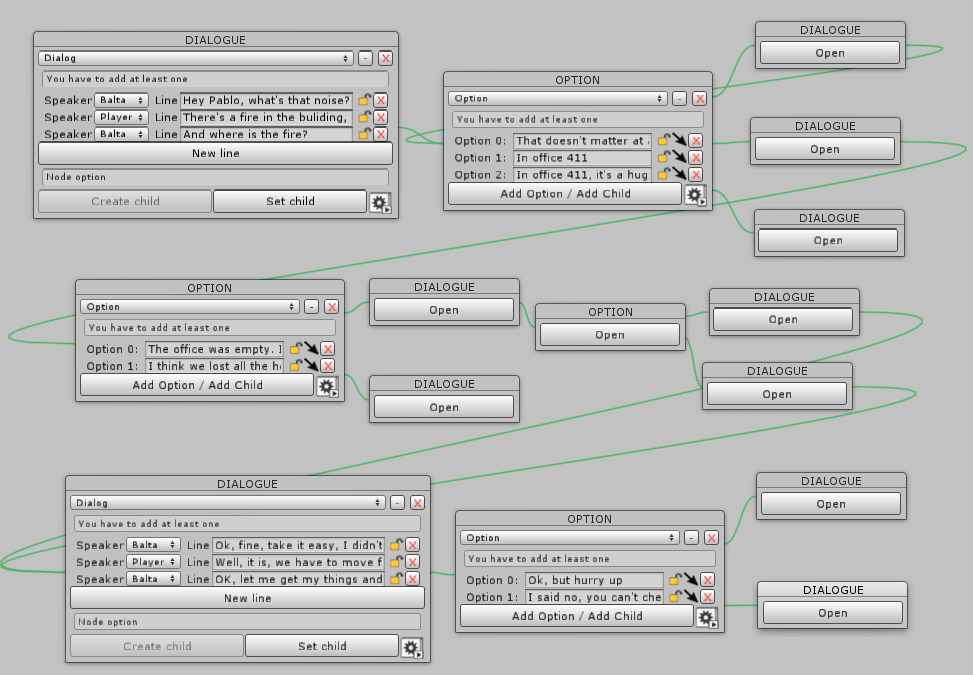
\includegraphics[height=3in]{figures/it3/big-dialog.png}}
	\caption[Gran diálogo - Editor de Diálogos]{Gran diálogo mostrado en el editor de diálogos.}
	\label{big-dialog-it3}
\end{figure}



% +-------------------------------------------------------------------------+
% | References                                                              |
% +-------------------------------------------------------------------------+

% +-------------------------------------------------------------------------+
% | In order for WinEDT to index references correctly, it has to know where |
% | the file resides.  The following command is prefaced by %, and will be  |
% | ignored completely by LaTeX.  However, WinEDT will use this line to     |
% | access the external .bib bibliography file.  Also note that WinEDT can  |
% | read file path names with either "\" or "/" - LaTeX, however, doesn't   |
% | like "\", so it's easier to store a path name in the "Unix" style.      |
% +-------------------------------------------------------------------------+

%Included for Gather Purpose only.  Do NOT uncomment:
%input "references.bib"

% +--------------------------------------------------------------------+
% | This template uses the BibTeX program to format references.  The
% | 3 lines below create a separate Bibliography section and add
% | an entry for "Bibliography" to the Table of Contents.  The actual
% | data for your references (author, title, journal, date, etc.) are
% | entered in the references.bib file.  See that file for information
% | on how to enter references.
% +--------------------------------------------------------------------+

\bibdata{references}
\bibliography{references}
\addcontentsline{toc}{chapter}{Bibliography}

% +--------------------------------------------------------------------+
% | Finally, we generate the appendix.  To add or delete appendices,
% | add or remove the line
% |
% |     \input{appendixX.tex}
% |
% | where "X" is the letter designation of the Appendix (A, B, C, etc.)
% | You should have one \input{appendixX.tex} line and a corresponding
% | file appendixX.tex for each appendix.                                 |
% +--------------------------------------------------------------------+

\appendix
% +--------------------------------------------------------------------+
% | Appendix A Page (Optional)                                         |
% +--------------------------------------------------------------------+

\cleardoublepage

\chapter{Title for This Appendix}
\label{Appendix:Key1}


% +--------------------------------------------------------------------+
% | Enter text for your Appendix page in the space below this box.     |
% |                                                                    |
% +--------------------------------------------------------------------+

% +--------------------------------------------------------------------+
% | Appendix B Page (Optional)                                         |
% +--------------------------------------------------------------------+

\cleardoublepage

\chapter{Title for This Appendix}
\label{Appendix:Key2}

% +--------------------------------------------------------------------+
% | Enter text for your Appendix page in the space below this box.     |
% |                                                                    |
% +--------------------------------------------------------------------+


\end{document}
